% +------------------------------------------------------------------------+
% | CBP Reference Manual:  main.tex
% +------------------------------------------------------------------------+
% | Automatically generated driver file for the reference manual chapter
% | of this package. Do not edit manually, you may loose your changes.
% +------------------------------------------------------------------------+

% +------------------------------------------------------------------------+
% | Reference manual page: Convex_hull_d_ref/intro.tex
% +------------------------------------------------------------------------+

%\clearpage
%\section{Reference Pages for dD Convex Hulls and Delaunay Triangulations}
\ccRefChapter{dD Convex Hulls and Delaunay Triangulations\label{chap:convex_hull_d_ref}}
\ccChapterAuthor{Susan Hert \and Michael Seel}

A subset $S \subseteq \R^3$ is convex if for any two points $p$ and $q$
in the set the line segment with endpoints $p$ and $q$ is contained
in $S$. The convex hull\ccIndexMainItemDef{convex hull} of a set $S$ is 
the smallest convex set containing
$S$. The convex hull of a set of points $P$ is a convex 
polytope with vertices in $P$.  A point in $P$ is an extreme point 
(with respect to $P$)\ccIndexMainItemDef{extreme point} if it is a vertex 
of the convex hull of $P$.

\cgal\ provides functions for computing convex hulls in two, three 
and arbitrary dimensions as well as functions for testing if a given set of 
points in is strongly convex or not.  This chapter describes the class
available for arbitrary dimensions and its companion class for 
computing the nearest and furthest side Delaunay triangulation. 

\section{Classified Reference Pages}

\ccHeading{Concepts}

\ccRefConceptPage{ConvexHullTraits_d} \\
\ccRefConceptPage{DelaunayLiftedTraits_d} \\
\ccRefConceptPage{DelaunayTraits_d} \\

\ccHeading{Classes}

\ccRefIdfierPage{CGAL::Convex_hull_d_traits_3<R>} \\
\ccRefIdfierPage{CGAL::Convex_hull_d<R>}  \\
\ccRefIdfierPage{CGAL::Delaunay_d< R, Lifted_R >} 

\clearpage




% +------------------------------------------------------------------------+
% | Reference manual page: ch_akl_toussaint.tex
% +------------------------------------------------------------------------+
% | 09.05.2001   Susan Hert and Stefan Schirra
% | Package: Convex_hull_2
% |
% +------------------------------------------------------------------------+

%\renewcommand{\ccRefPageBegin}{\begin{ccAdvanced}}
%\renewcommand{\ccRefPageEnd}{\end{ccAdvanced}}
\begin{ccRefFunction}{ch_akl_toussaint}  %% add template arg's if necessary
\ccIndexSubitemBegin{convex hull, 2D}{Akl-Toussaint algorithm}

\ccDefinition
  
The function \ccRefName\ generates the counterclockwise sequence of extreme
points from a given set of input points.


\ccInclude{CGAL/ch_akl_toussiant.h}

\ccFunction{template <class ForwardIterator, class OutputIterator, class Traits>
            OutputIterator
            ch_akl_toussaint(ForwardIterator first, ForwardIterator beyond,
                             OutputIterator  result,
                             const Traits& ch_traits = Default_traits());}
            {generates the counterclockwise sequence of extreme points
            of the points in the range [\ccc{first},\ccc{beyond}).
            The resulting sequence is placed starting at position
            \ccc{result}, and the past-the-end iterator for the resulting
            sequence is returned. It is not specified at which point the
            cyclic sequence of extreme points is cut into a linear sequence.
            \ccPrecond %\ccIndexSubitem[C]{ch_akl_toussaint}{preconditions}
            The source range [\ccc{first},\ccc{beyond}) does not contain
            \ccc{result}.}


The default traits class \ccc{Default_traits} is the kernel in which the
type \ccc{ForwardIteartor::value_type} is defined.

\ccHeading{Requirements}
\begin{enumerate}
   \item    \ccc{ForwardIterator::value_type} and 
            \ccc{OutputIterator::value_type}
            are equivalent to \ccc{Traits::Point_2}.
   \item    \ccc{Traits} defines the following subset of types from
            the concept ConvexHullTraits\_2 and their corresponding member
            %\ccIndexMainItem[c]{ConvexHullTraits_2}
            functions that return instances of these types:
            \begin{itemize}
                \item \ccc{Traits::Point_2},
                \item \ccc{Traits::Less_xy_2}, 
                \item \ccc{Traits::Less_yx_2},
                \item \ccc{Traits::Leftturn_2}.
            \end{itemize}
\end{enumerate}


\ccSeeAlso

\ccRefIdfierPage{CGAL::ch_bykat} \\
\ccRefIdfierPage{CGAL::ch_eddy} \\
\ccRefIdfierPage{CGAL::ch_graham_andrew} \\
\ccRefIdfierPage{CGAL::ch_jarvis} \\
\ccRefIdfierPage{CGAL::ch_melkman} \\
\ccRefIdfierPage{CGAL::convex_hull_2} 

\ccImplementation

This function uses the algorithm of Akl and
Toussaint \cite{at-fcha-78} that requires $O(n \log n)$ time for $n$ input
points.  

\ccIndexSubitemEnd{convex hull, 2D}{Akl-Toussaint algorithm}
\end{ccRefFunction}
%\renewcommand{\ccRefPageBegin}{}
%\renewcommand{\ccRefPageEnd}{}

% +------------------------------------------------------------------------+
%%RefPage: end of main body, begin of footer
% EOF
% +------------------------------------------------------------------------+


% +------------------------------------------------------------------------+
% | Reference manual page: ch_bykat.tex
% +------------------------------------------------------------------------+
% | 09.05.2001   Susan Hert and Stefan Schirra
% | Package: Convex_hull_2
% | 
% +------------------------------------------------------------------------+

%\renewcommand{\ccRefPageBegin}{\begin{ccAdvanced}}
%\renewcommand{\ccRefPageEnd}{\end{ccAdvanced}}
\begin{ccRefFunction}{ch_bykat}  
\ccIndexSubitemBegin{convex hull, 2D}{Bykat algorithm}

\ccDefinition
  
The function \ccRefName\ generates the counterclockwise sequence of extreme
points from a given set of input points.


\ccInclude{CGAL/ch_bykat.h}

\ccFunction{template <class InputIterator, class OutputIterator, class Traits>
            OutputIterator
            ch_bykat( InputIterator  first,
                              InputIterator  beyond,
                              OutputIterator result,
                              const Traits & ch_traits = Default_traits);}
            {generates the counterclockwise sequence of extreme points
            of the points in the range [\ccc{first},\ccc{beyond}).
            The resulting sequence is placed starting at position
            \ccc{result}, and the past-the-end iterator for the resulting
            sequence is returned. It is not specified at which point the
            cyclic sequence of extreme points is cut into a linear sequence.
            \ccPrecond{ %\ccIndexSubitem[C]{ch_bykat}{preconditions}
            The source range [\ccc{first},\ccc{beyond}) does not contain
            \ccc{result}.}}

The default traits class \ccc{Default_traits} is the kernel in which the
type \ccc{ForwardIterator::value_type} is defined.


\ccHeading{Requirements}
\begin{enumerate}
   \item    \ccc{InputIterator::value_type} and 
            \ccc{OutputIterator::value_type}
            are equivalent to \ccc{Traits::Point_2}.
   \item    \ccc{Traits} defines the following subset of types from
            the concept \ccc{ConvexHullTraits_2} and their corresponding member
            %\ccIndexMainItem[c]{ConvexHullTraits_2}
            functions that return instances of these types:
            \begin{itemize}
                \item \ccc{Traits::Point_2},
                \item \ccc{Traits::Less_signed_distance_to_line_2},
                \item \ccc{Traits::Left_turn_2}, 
                \item \ccc{Traits::Less_xy_2},
		\item \ccc{Traits::Equal_2}.
            \end{itemize}
\end{enumerate}

\ccSeeAlso

\ccRefIdfierPage{CGAL::ch_akl_toussaint} \\
\ccRefIdfierPage{CGAL::ch_eddy} \\
\ccRefIdfierPage{CGAL::ch_graham_andrew} \\
\ccRefIdfierPage{CGAL::ch_jarvis} \\
\ccRefIdfierPage{CGAL::ch_melkman} \\
\ccRefIdfierPage{CGAL::convex_hull_2} 

\ccImplementation
This function implements the non-recursive variation of
Eddy's algorithm \cite{e-nchap-77} described in \cite{b-chfsp-78}.
This algorithm requires $O(n h)$ time 
in the worst case for $n$ input points with $h$ extreme points.  

\ccIndexSubitemEnd{convex hull, 2D}{Bykat algorithm}
\end{ccRefFunction}
%\renewcommand{\ccRefPageBegin}{}
%\renewcommand{\ccRefPageEnd}{}

% +------------------------------------------------------------------------+
%%RefPage: end of main body, begin of footer
% EOF
% +------------------------------------------------------------------------+


% +------------------------------------------------------------------------+
% | Reference manual page: ch_eddy.tex
% +------------------------------------------------------------------------+
% | 09.05.2001   Susan Hert and Stefan Schirra
% | Package: Convex_hull_2
% | 
% +------------------------------------------------------------------------+

%\renewcommand{\ccRefPageBegin}{\begin{ccAdvanced}}
%\renewcommand{\ccRefPageEnd}{\end{ccAdvanced}}
\begin{ccRefFunction}{ch_eddy}  %% add template arg's if necessary
\ccIndexSubitemBegin{convex hull, 2D}{Eddy algorithm}

\ccDefinition
  
The function \ccRefName\ generates the counterclockwise sequence of extreme
points from a given set of input points using Eddy's algorithm 
\cite{e-nchap-77}.  This is the two-dimensional version of the quickhull
algorithm \cite{bdh-qach-96}%
\ccIndexMainItem{quickhull, 2D}
\ccIndexSubitem{convex hull, 2D}{quickhull}. 
This algorithm requires $O(n h)$ time 
in the worst case for $n$ input points with $h$ extreme points.  

\ccInclude{CGAL/ch_eddy.h}

\ccFunction{template <class InputIterator, class OutputIterator, class Traits>
            OutputIterator
            ch_eddy( InputIterator  first,
                     InputIterator  beyond,
                     OutputIterator result,
                     const Traits & ch_traits = Default_traits);}
            {generates the counterclockwise sequence of extreme points
            of the points in the range [\ccc{first},\ccc{beyond}).
            The resulting sequence is placed starting at position
            \ccc{result}, and the past-the-end iterator for the resulting
            sequence is returned. It is not specified at which point the
            cyclic sequence of extreme points is cut into a linear sequence.
            \ccPrecond %\ccIndexSubitem[C]{ch_eddy}{preconditions}
            The source range [\ccc{first},\ccc{beyond}) does not contain
            \ccc{result}.}

The default traits class \ccc{Default_traits} is the \cgal\
\ccc{Kernel_traits_2} class,%\ccIndexTraitsClassDefault{ch_eddy}
with the representation type determined by \ccc{ForwardIteartor::value_type}.


\ccHeading{Requirements}
\begin{enumerate}
   \item    \ccc{InputIterator::value_type} and 
            \ccc{OutputIterator::value_type}
            should be \ccc{Traits::Point_2}.
   \item    \ccc{Traits} defines the following subset of types from
            the concept ConvexHullTraits\_2 and their corresponding member
            %\ccIndexMainItem[c]{ConvexHullTraits_2}
            functions that return instances of these types:
            \begin{itemize}
                \item \ccc{Traits::Point_2},
                \item \ccc{Traits::Less_signed_distance_to_line_2},
                \item \ccc{Traits::Left_of_line_2}, 
                \item \ccc{Traits::Less_xy_2}.
            \end{itemize}
\end{enumerate}

\ccSeeAlso

\ccRefIdfierPage{CGAL::ch_akl_toussaint} \\
\ccRefIdfierPage{CGAL::ch_bykat} \\
\ccRefIdfierPage{CGAL::ch_graham_andrew} \\
\ccRefIdfierPage{CGAL::ch_jarvis} \\
\ccRefIdfierPage{CGAL::ch_melkman} \\
\ccRefIdfierPage{CGAL::convex_hull_2} 

\ccIndexSubitemEnd{convex hull, 2D}{Eddy algorithm}
\end{ccRefFunction}
%\renewcommand{\ccRefPageBegin}{}
%\renewcommand{\ccRefPageEnd}{}

% +------------------------------------------------------------------------+
%%RefPage: end of main body, begin of footer
% EOF
% +------------------------------------------------------------------------+


% +------------------------------------------------------------------------+
% | Reference manual page: ch_e_point.tex
% +------------------------------------------------------------------------+
% | 09.05.2001   Susan Hert and Stefan Schirra
% | Package: Convex_hull_2
% | 
% +------------------------------------------------------------------------+


\begin{ccRefFunction}{ch_e_point}  %% add template arg's if necessary
\ccIndexSubitemBegin{extreme points, 2D}{in coordinate directions}

\ccDefinition
  
The function \ccRefName\ finds a point of a given set  
of input points with maximal $x$ coordinate.

\ccInclude{CGAL/ch_selected_extreme_points_2.h}

\ccFunction{template <class ForwardIterator>
            void
            ch_e_point( ForwardIterator first, ForwardIterator beyond,
                        ForwardIterator& e,
                        const Traits & ch_traits = Default_traits);}
           {traverses the range [\ccc{first},\ccc{beyond}).
            After execution, the value of
            \ccc{e} is an iterator in the range such that \ccc{*e} $\ge_{xy}$
            \ccc{*it} for all iterators \ccc{it} in the range. }

The default traits class \ccc{Default_traits} is the kernel in which the
type \ccc{ForwardIterator::value_type} is defined.

\ccHeading{Requirements}
\ccc{Traits} defines a type \ccc{Traits::Less_xy_2} as described in 
the concept ConvexHullTraits\_2 and the corresponding member
%\ccIndexMainItem[c]{ConvexHullTraits_2}
function that returns an instance of this type.



\ccSeeAlso

\ccRefIdfierPage{CGAL::ch_nswe_point} \\
\ccRefIdfierPage{CGAL::ch_n_point} \\
\ccRefIdfierPage{CGAL::ch_ns_point} \\
\ccRefIdfierPage{CGAL::ch_s_point} \\
\ccRefIdfierPage{CGAL::ch_w_point} \\
\ccRefIdfierPage{CGAL::ch_we_point} 

\ccIndexSubitemEnd{extreme points, 2D}{in coordinate directions}
\end{ccRefFunction}

% +------------------------------------------------------------------------+
%%RefPage: end of main body, begin of footer
% EOF
% +------------------------------------------------------------------------+


% +------------------------------------------------------------------------+
% | Reference manual page: ch_graham_andrew.tex
% +------------------------------------------------------------------------+
% | 09.05.2001   Susan Hert and Stefan Schirra
% | Package: Convex_hull_2
% | 
% +------------------------------------------------------------------------+

%\renewcommand{\ccRefPageBegin}{\begin{ccAdvanced}}
%\renewcommand{\ccRefPageEnd}{\end{ccAdvanced}}
\begin{ccRefFunction}{ch_graham_andrew}  %% add template arg's if necessary
\ccIndexSubitemBegin{convex hull, 2D}{Graham-Andrew scan}

\ccDefinition
  
The function \ccRefName\ generates the counterclockwise sequence of extreme
points from a given set of input points using Andrew's variant of the Graham
scan algorithm \cite{a-aeach-79} and follows the presenation of Mehlhorn
\cite{m-mdscg-84}. This algorithm requires $O(n \log n)$ time 
in the worst case for $n$ input points.  

\ccInclude{CGAL/ch_graham_andrew.h}

\ccFunction{template <class InputIterator, class OutputIterator, class Traits>
            OutputIterator
            ch_graham_andrew( InputIterator  first,
                              InputIterator  beyond,
                              OutputIterator result,
                              const Traits & ch_traits = Default_traits);}
            {generates the counterclockwise sequence of extreme points
            of the points in the range [\ccc{first},\ccc{beyond}).
            The resulting sequence is placed starting at position
            \ccc{result}, and the past-the-end iterator for the resulting
            sequence is returned. It is not specified at which point the
            cyclic sequence of extreme points is cut into a linear sequence.
            \ccPrecond %\ccIndexSubitem[C]{ch_graham_andrew}{preconditions}
            The source range [\ccc{first},\ccc{beyond}) does not contain
            \ccc{result}.}

The default traits class \ccc{Default_traits} is the \cgal\
\ccc{Kernel_traits_2} class,%\ccIndexTraitsClassDefault{ch_graham_andrew}
with the representation type determined by \ccc{ForwardIteartor::value_type}.

\ccHeading{Requirements}
\begin{enumerate}
   \item    \ccc{InputIterator::value_type} and 
            \ccc{OutputIterator::value_type}
            should be \ccc{Traits::Point_2}.
   \item    \ccc{Traits} defines the following subset of types from
            the concept ConvexHullTraits\_2 and their corresponding member
            %\ccIndexMainItem[c]{ConvexHullTraits_2}
            functions that return instances of these types:
            \begin{itemize}
                \item \ccc{Traits::Point_2},
                \item \ccc{Traits::Less_xy_2}, 
                \item \ccc{Traits::Leftturn_2}.
            \end{itemize}
\end{enumerate}

\ccSeeAlso

\ccRefIdfierPage{CGAL::ch_akl_toussaint} \\
\ccRefIdfierPage{CGAL::ch_bykat} \\
\ccRefIdfierPage{CGAL::ch_eddy} \\
\ccRefIdfierPage{CGAL::ch_graham_andrew_scan} \\
\ccRefIdfierPage{CGAL::ch_jarvis} \\
\ccRefIdfierPage{CGAL::ch_melkman} \\
\ccRefIdfierPage{CGAL::convex_hull_points_2} \\
\ccRefIdfierPage{CGAL::lower_hull_points_2} \\
\ccRefIdfierPage{CGAL::upper_hull_points_2} 

\ccIndexSubitemEnd{convex hull, 2D}{Graham-Andrew scan}
\end{ccRefFunction}
%\renewcommand{\ccRefPageBegin}{}
%\renewcommand{\ccRefPageEnd}{}

% +------------------------------------------------------------------------+
%%RefPage: end of main body, begin of footer
% EOF
% +------------------------------------------------------------------------+


% +------------------------------------------------------------------------+
% | Reference manual page: ch_graham_andrew.tex
% +------------------------------------------------------------------------+
% | 09.05.2001   Susan Hert and Stefan Schirra
% | Package: Convex_hull_2
% |
% +------------------------------------------------------------------------+


\begin{ccRefFunction}{ch_graham_andrew_scan}  %% add template arg's if necessary
\ccIndexSubitemBegin{convex hull, 2D}{Graham-Andrew scan}
\ccIndexSubitemBegin{extreme points, 2D}{right of line}

\ccDefinition
  
The function \ccRefName\ generates the counterclockwise sequence of extreme
points from a given set of input points that are not left of the line defined
by the first and last points in this sequence.  


\ccInclude{CGAL/ch_graham_andrew.h}

\ccFunction{template <class BidirectionalIterator, class OutputIterator, 
                      class Traits>
            OutputIterator
            ch_graham_andrew_scan( BidirectionalIterator first,
                                   BidirectionalIterator beyond,
                                   OutputIterator        result,
                                   const Traits& ch_traits = Default_traits);}
           {generates the counterclockwise sequence of extreme points that are
            not left of $pq$, where $p$ is the value of \ccc{first} and $q$ is
            the value of \ccc{beyond} $-1$. The resulting sequence is placed
            starting at \ccc{result} with $p$; point $q$ is omitted.  The
            past-the-end iterator for the sequence is returned.
            \ccPrecond %\ccIndexSubitem[C]{ch_graham_andrew_scan}{preconditions}
            The range [\ccc{first},\ccc{beyond}) contains at least
            two different points.
            The points in [\ccc{first},\ccc{beyond}) are ``sorted'' with respect
            to $pq$, {\it i.e.}, the sequence of points in 
            [\ccc{first},\ccc{beyond}) define a counterclockwise polygon, 
            for which the Graham-Sklansky-procedure \cite{s-mcrm-72} works.}

The default traits class \ccc{Default_traits} is the kernel in which the
type \ccc{BidirectionalIterator::value_type} is defined.


\ccHeading{Requirements}
\begin{enumerate}
   \item    \ccc{BidirectionalIterator::value_type} and 
            \ccc{OutputIterator::value_type}
            are equivalent to \ccc{Traits::Point_2}.
   \item    \ccc{Traits} defines the following two types from
            the concept ConvexHullTraits\_2 and their corresponding member
            %\ccIndexMainItem[c]{ConvexHullTraits_2}
            functions that return instances of these types:
            \begin{itemize}
                \item \ccc{Traits::Point_2},
                \item \ccc{Traits::Left_turn_2}.
            \end{itemize}
\end{enumerate}


\ccSeeAlso

\ccRefIdfierPage{CGAL::ch_graham_andrew} \\
\ccRefIdfierPage{CGAL::lower_hull_points_2} \\
\ccRefIdfierPage{CGAL::upper_hull_points_2} 

\ccImplementation

The function uses Andrew's 
variant of the Graham scan algorithm \cite{a-aeach-79} . This algorithm 
requires $O(n \log n)$ time in the worst case for $n$ input points.  

\ccExample

In the following example \ccc{ch_graham_andrew_scan()} is used to
realize Anderson's variant \cite{a-readc-78} of the Graham Scan 
\cite{g-eadch-72}.  The points are sorted counterclockwise around the leftmost 
point using the \ccc{Less_rotate_ccw_2} predicate, as defined in
the concept ConvexHullTraits\_2. According to the definition 
of \ccc{Less_rotate_ccw_2}, the leftmost point is the last point in the sorted 
sequence and its predecessor on the convex hull is the first point in the 
sorted sequence.  It is not hard to see that the preconditions of
\ccc{ch_graham_andrew_scan()} are satisfied.  Anderson's variant of the 
Graham scan is usually inferior to Andrew's variant because of its higher 
arithmetic demand.

\begin{verbatim}
template <class InputIterator, class OutputIterator, class Traits>
OutputIterator
ch_graham_anderson( InputIterator  first, InputIterator  beyond,
                    OutputIterator result, const Traits&  ch_traits)
{
  typedef typename Traits::Less_xy_2          Less_xy_2;
  typedef typename Traits::Point_2            Point_2;
  typedef typename Traits::Less_rotate_ccw_2  Less_rotate_ccw_2;

  if (first == beyond) return result;
  std::vector< Point_2 >  V;
  copy( first, beyond, back_inserter(V) );
  typename std::vector< Point_2 >::iterator it = 
               std::min_element(V.begin(), V.end(), Less_xy_2());
  std::sort( V.begin(), V.end(), Less_rotate_ccw_2(*it) );
  if ( *(V.begin()) == *(V.rbegin()) )
  {
      *result = *(V.begin());  ++result;
      return result;
  }
  return ch_graham_andrew_scan( V.begin(), V.end(), result, ch_traits);
}
\end{verbatim}


\ccIndexSubitemEnd{convex hull, 2D}{Graham-Andrew scan}
\ccIndexSubitemEnd{extreme points, 2D}{right of line}
\end{ccRefFunction}

% +------------------------------------------------------------------------+
%%RefPage: end of main body, begin of footer
% EOF
% +------------------------------------------------------------------------+


% +------------------------------------------------------------------------+
% | Reference manual page: ch_jarvis.tex
% +------------------------------------------------------------------------+
% | 09.05.2001   Susan Hert and Stefan Schirra
% | Package: Convex_hull_2
% | 
% +------------------------------------------------------------------------+

%\renewcommand{\ccRefPageBegin}{\begin{ccAdvanced}}
%\renewcommand{\ccRefPageEnd}{\end{ccAdvanced}}
\begin{ccRefFunction}{ch_jarvis}  %% add template arg's if necessary
\ccIndexSubitemBegin{convex hull, 2D}{Jarvis march}
\ccIndexSubitemBegin{convex hull, 2D}{gift-wrapping}

\ccDefinition
  
The function \ccRefName\ generates the counterclockwise sequence of extreme
points from a given set of input points.


\ccInclude{CGAL/ch_jarvis.h}

\ccFunction{template <class InputIterator, class OutputIterator, class Traits>
            OutputIterator
            ch_jarvis( InputIterator  first,
                       InputIterator  beyond,
                       OutputIterator result,
                       const Traits & ch_traits = Default_traits);}
            {generates the counterclockwise sequence of extreme points
            of the points in the range [\ccc{first},\ccc{beyond}).
            The resulting sequence is placed starting at position
            \ccc{result}, and the past-the-end iterator for the resulting
            sequence is returned. It is not specified at which point the
            cyclic sequence of extreme points is cut into a linear sequence.
            \ccPrecond %\ccIndexSubitem[C]{ch_jarvis}{preconditions}
            The source range [\ccc{first},\ccc{beyond}) does not contain
            \ccc{result}.}

The default traits class \ccc{Default_traits} is the kernel in which the
type \ccc{InputIterator::value_type} is defined.

\ccHeading{Requirements}
\begin{enumerate}
   \item    \ccc{InputIterator::value_type} and 
            \ccc{OutputIterator::value_type}
            should be \ccc{Traits::Point_2}.
   \item    \ccc{Traits} defines the following subset of types from
            the concept ConvexHullTraits\_2 and their corresponding member
            %\ccIndexMainItem[c]{ConvexHullTraits_2}
            functions that return instances of these types:
            \begin{itemize}
                \item \ccc{Traits::Point_2},
                \item \ccc{Traits::Less_rotate_ccw_2},
                \item \ccc{Traits::Less_xy_2}.
            \end{itemize}
\end{enumerate}


\ccSeeAlso

\ccRefIdfierPage{CGAL::ch_akl_toussaint} \\
\ccRefIdfierPage{CGAL::ch_bykat} \\
\ccRefIdfierPage{CGAL::ch_eddy} \\
\ccRefIdfierPage{CGAL::ch_graham_andrew} \\
\ccRefIdfierPage{CGAL::ch_jarvis_march} \\
\ccRefIdfierPage{CGAL::ch_melkman} \\
\ccRefIdfierPage{CGAL::convex_hull_2} 

\ccIndexSubitemEnd{convex hull, 2D}{gift-wrapping}
\ccIndexSubitemEnd{convex hull, 2D}{Jarvis march}

\ccImplementation
This function uses the Jarvis march (gift-wrapping)
algorithm \cite{j-ichfs-73}. This algorithm requires $O(n h)$ time 
in the worst case for $n$ input points with $h$ extreme points.  

\end{ccRefFunction}
%\renewcommand{\ccRefPageBegin}{}
%\renewcommand{\ccRefPageEnd}{}

% +------------------------------------------------------------------------+
%%RefPage: end of main body, begin of footer
% EOF
% +------------------------------------------------------------------------+


% +------------------------------------------------------------------------+
% | Reference manual page: ch_jarvis_march.tex
% +------------------------------------------------------------------------+
% | 09.05.2001   Susan Hert and Stefan Schirra
% | Package: Convex_hull_2
% |
% +------------------------------------------------------------------------+

\begin{ccRefFunction}{ch_jarvis_march}  %% add template arg's if necessary
\ccIndexSubitemBegin{convex hull, 2D}{Jarvis march}
\ccIndexSubitemBegin{convex hull, 2D}{gift-wrapping}
\ccIndexSubitemBegin{extreme points, 2D}{between two points}

\ccDefinition
  
The function \ccRefName\ generates the counterclockwise sequence of extreme
points from a given set of input points that line between two input points.


\ccInclude{CGAL/ch_jarvis.h}

\ccFunction{template <class ForwardIterator, class OutputIterator, class Traits>
            OutputIterator
            ch_jarvis_march(ForwardIterator first, ForwardIterator beyond,
                            const Traits::Point_2& start_p,
                            const Traits::Point_2& stop_p,
                            OutputIterator  result,
                            const Traits& ch_traits = Default_traits);}
            {generates the counterclockwise subsequence of
             extreme points between \ccc{start_p} and \ccc{stop_p} of the 
             points in the range [\ccc{first},\ccc{beyond}), starting at 
             position \ccc{result} with point \ccc{start_p}.  The last point 
             generated is the point preceding \ccc{stop_p} in the 
             counterclockwise order of extreme points.\\
            \ccPrecond%\ccIndexSubitem[C]{ch_jarvis_march}{preconditions}
            \ccc{start_p} and \ccc{stop_p} are extreme points with respect to
            the points in the range [\ccc{first},\ccc{beyond}) and \ccc{stop_p}
            is an element of range [\ccc{first},\ccc{beyond}).}


The default traits class \ccc{Default_traits} is the kernel in which the
type \ccc{ForwardIterator::value_type} is defined.


\ccHeading{Requirements}
\begin{enumerate}
   \item    \ccc{ForwardIterator::value_type} and 
            \ccc{OutputIterator::value_type}
            are equivalent to \ccc{Traits::Point_2}.
   \item    \ccc{Traits} defines the following subset of types from
            the concept ConvexHullTraits\_2 and their corresponding member
            %\ccIndexMainItem[c]{ConvexHullTraits_2}
            functions that return instances of these types:
            \begin{itemize}
                \item \ccc{Traits::Point_2},
		\item \ccc{Traits::Equal_2},
                \item \ccc{Traits::Less_rotate_ccw_2}.
            \end{itemize}
\end{enumerate}

\ccSeeAlso

\ccRefIdfierPage{CGAL::ch_jarvis} \\
\ccRefIdfierPage{CGAL::lower_hull_points_2} \\
\ccRefIdfierPage{CGAL::upper_hull_points_2} \\

\ccIndexSubitemEnd{convex hull, 2D}{Jarvis march}
\ccIndexSubitemEnd{convex hull, 2D}{gift-wrapping}
\ccIndexSubitemEnd{extreme points, 2D}{between two points}

\ccImplementation

The function uses the Jarvis march (gift-wrapping)
algorithm \cite{j-ichfs-73}. This algorithm requires $O(n h)$ time 
in the worst case for $n$ input points with $h$ extreme points.  
\end{ccRefFunction}

% +------------------------------------------------------------------------+
%%RefPage: end of main body, begin of footer
% EOF
% +------------------------------------------------------------------------+


% +------------------------------------------------------------------------+
% | Reference manual page: ch_melkman.tex
% +------------------------------------------------------------------------+
% | 09.05.2001   Susan Hert and Stefan Schirra
% | Package: Convex_hull_2
% | 
% +------------------------------------------------------------------------+


\begin{ccRefFunction}{ch_melkman}  %% add template arg's if necessary
\ccIndexSubitemBegin{convex hull, 2D}{of polyline or polygon}
\ccIndexSubitemBegin{convex hull, 2D}{Melkman algorithm}

\ccDefinition
  
The function \ccRefName\ computes the counterclockwise sequence of
extreme points of a sequence of points that forms a simple polyline or polygon.

\ccInclude{CGAL/ch_melkman.h}

\ccFunction{template <class InputIterator, class OutputIterator>
            OutputIterator
            ch_melkman( InputIterator first, InputIterator last,  
                        OutputIterator result, 
                        const Traits& ch_traits = Default_traits);}
            {generates the counterclockwise sequence of extreme points
            of the points in the range [\ccc{first}, \ccc{beyond}). 
            The resulting sequence is placed starting at
            position \ccc{result}, and the past-the-end iterator for
            the resulting sequence is returned.
            \ccPrecond %\ccIndexSubitem[C]{ch_melkman}{preconditions}
            The source range [\ccc{first},\ccc{beyond}) corresponds 
            to a simple polyline. 
            [\ccc{first},\ccc{beyond}) does not contain \ccc{result}}.

The default traits class \ccc{Default_traits} is the kernel in which the
type \ccc{InputIterator::value_type} is defined.


\ccHeading{Requirements}
\begin{enumerate}
   \item    \ccc{InputIterator::value_type} and \ccc{OutputIterator::value_type}
            are equivalent to \ccc{Traits::Point_2}.
   \item    \ccc{Traits} contains the following subset of types from
            the concept ConvexHullTraits\_2 and their corresponding member
            %\ccIndexMainItem[c]{ConvexHullTraits_2}
            functions that return instances of these types:
            \begin{itemize}
                \item \ccc{Traits::Point_2},
                \item \ccc{Traits::Less_xy_2}, 
                \item \ccc{Traits::Left_turn_2}.
            \end{itemize}
\end{enumerate}

\ccSeeAlso

\ccRefIdfierPage{CGAL::ch_akl_toussaint} \\
\ccRefIdfierPage{CGAL::ch_bykat} \\
\ccRefIdfierPage{CGAL::ch_eddy} \\
\ccRefIdfierPage{CGAL::ch_graham_andrew} \\
\ccRefIdfierPage{CGAL::ch_jarvis} \\
\ccRefIdfierPage{CGAL::ch_melkman} \\
\ccRefIdfierPage{CGAL::convex_hull_2} 

\ccImplementation

It uses an implementation of Melkman's algorithm \cite{m-olcch-87}. Running
time of this is linear.

\ccIndexSubitemEnd{convex hull, 2D}{of polyline or polygon}
\ccIndexSubitemEnd{convex hull, 2D}{Melkman algorithm}
\end{ccRefFunction}

% +------------------------------------------------------------------------+
%%RefPage: end of main body, begin of footer
% EOF
% +------------------------------------------------------------------------+


% +------------------------------------------------------------------------+
% | Reference manual page: ch_nswe_point.tex
% +------------------------------------------------------------------------+
% | 09.05.2001   Susan Hert and Stefan Schirra
% | Package: Convex_hull_2
% | 
% +------------------------------------------------------------------------+


\begin{ccRefFunction}{ch_nswe_point}  %% add template arg's if necessary
\ccIndexSubitemBegin{extreme points, 2D}{in coordinate directions}

\ccDefinition
  
The function \ccRefName\ finds the four extreme points of a given set  
of input points using a linear scan of the input points.  
That is, it determines the points with maximal $y$, minimal $y$,
minimal $x$, and maximal $x$ coordinates.

\ccInclude{CGAL/ch_selected_extreme_points_2.h}

\ccFunction{template <class ForwardIterator>
            void
            ch_nswe_point( ForwardIterator first, ForwardIterator beyond,
                           ForwardIterator& n,
                           ForwardIterator& s,
                           ForwardIterator& w,
                           ForwardIterator& e,
                           const Traits & ch_traits = Default_traits);}
           {traverses the range [\ccc{first},\ccc{beyond}).
            After execution, the value of
            \ccc{n} is an iterator in the range such that \ccc{*n} $\ge_{yx}$
            \ccc{*it} for all iterators \ccc{it} in the range. Similarly, for
            \ccc{s}, \ccc{w}, and \ccc{e} the inequalities \ccc{*s} $\le_{yx}$
            \ccc{*it}, \ccc{*w} $\le_{xy}$ \ccc{*it}, and \ccc{*e}
            $\ge_{xy}$ \ccc{*it} hold for all iterators
            \ccc{it} in the range.}


\ccHeading{Requirements}
\ccc{Traits} contains the following subset of types from
the concept ConvexHullTraits\_2 and their corresponding member
functions that return instances of these types:
            \begin{itemize}
                \item \ccc{Traits::Less_xy_2}, 
                \item \ccc{Traits::Less_yx_2}.
            \end{itemize}

The default traits class \ccc{Default_traits} is the \cgal\ 
\ccc{Kernel_traits_2} class,
with the representation type determined by \ccc{ForwardIteartor::value_type}.


\ccSeeAlso

\ccRefIdfierPage{CGAL::ch_e_point} \\
\ccRefIdfierPage{CGAL::ch_n_point} \\
\ccRefIdfierPage{CGAL::ch_ns_point} \\
\ccRefIdfierPage{CGAL::ch_s_point} \\
\ccRefIdfierPage{CGAL::ch_w_point} \\
\ccRefIdfierPage{CGAL::ch_we_point} 

\ccIndexSubitemEnd{extreme points, 2D}{in coordinate directions}
\end{ccRefFunction}

% +------------------------------------------------------------------------+
%%RefPage: end of main body, begin of footer
% EOF
% +------------------------------------------------------------------------+


% +------------------------------------------------------------------------+
% | Reference manual page: ch_ns_point.tex
% +------------------------------------------------------------------------+
% | 09.05.2001   Susan Hert and Stefan Schirra
% | Package: Convex_hull_2
% | 
% +------------------------------------------------------------------------+


\begin{ccRefFunction}{ch_ns_point}  %% add template arg's if necessary
\ccIndexSubitemBegin{extreme points, 2D}{in coordinate directions}

\ccDefinition
  
The function \ccRefName\ finds the points of a given set  
of input points with minimal and maximal $x$ coordinates.

\ccInclude{CGAL/ch_selected_extreme_points_2.h}

\ccFunction{template <class ForwardIterator>
            void
            ch_ns_point( ForwardIterator first, ForwardIterator beyond,
                         ForwardIterator& n,
                         ForwardIterator& s,
                         const Traits & ch_traits = Default_traits);}
           {traverses the range [\ccc{first},\ccc{beyond}).
            After execution, the value of
            \ccc{n} is an iterator in the range such that \ccc{*n} $\ge_{yx}$
            \ccc{*it} for all iterators \ccc{it} in the range. Similarly, for
            \ccc{s} the inequality \ccc{*s} $\le_{yx}$ \ccc{*it}
            holds for all iterators in the range.}

The default traits class \ccc{Default_traits} is the kernel in which the
type \ccc{ForwardIterator::value_type} is defined.


\ccHeading{Requirements}
\ccc{Traits} defines the type \ccc{Traits::Less_yx_2} as specified in
the concept \ccc{ConvexHullTraits_2} and the corresponding member
function that returns an instance of this type.


\ccSeeAlso

\ccRefIdfierPage{CGAL::ch_e_point} \\
\ccRefIdfierPage{CGAL::ch_nswe_point} \\
\ccRefIdfierPage{CGAL::ch_n_point} \\
\ccRefIdfierPage{CGAL::ch_s_point} \\
\ccRefIdfierPage{CGAL::ch_w_point} \\
\ccRefIdfierPage{CGAL::ch_we_point} 

\ccIndexSubitemEnd{extreme points, 2D}{in coordinate directions}
\end{ccRefFunction}

% +------------------------------------------------------------------------+
%%RefPage: end of main body, begin of footer
% EOF
% +------------------------------------------------------------------------+


% +------------------------------------------------------------------------+
% | Reference manual page: ch_n_point.tex
% +------------------------------------------------------------------------+
% | 09.05.2001   Susan Hert and Stefan Schirra
% | Package: Convex_hull_2
% | 
% +------------------------------------------------------------------------+


\begin{ccRefFunction}{ch_n_point}  %% add template arg's if necessary
\ccIndexSubitemBegin{extreme points, 2D}{in coordinate directions}

\ccDefinition
  
The function \ccRefName\ finds a point in a given set  
of input points with maximal $y$ coordinate.

\ccInclude{CGAL/ch_selected_extreme_points_2.h}

\ccFunction{template <class ForwardIterator>
            void
            ch_n_point( ForwardIterator first, ForwardIterator beyond,
                        ForwardIterator& n,
                        const Traits & ch_traits = Default_traits);}
           {traverses the range [\ccc{first},\ccc{beyond}).
            After execution, the value of
            \ccc{n} is an iterator in the range such that \ccc{*n} $\ge_{yx}$
            \ccc{*it} for all iterators \ccc{it} in the range.}


The default traits class \ccc{Default_traits} is the \cgal\ 
\ccc{Kernel_traits_2} class,
with the representation type determined by \ccc{ForwardIteartor::value_type}.

\ccHeading{Requirements}
\ccc{Traits} defines the type \ccc{Traits::Less_yx_2} as specified in
the concept ConvexHullTraits\_2 and the corresponding member
function that returns an instance of this type.


\ccSeeAlso

\ccRefIdfierPage{CGAL::ch_e_point} \\
\ccRefIdfierPage{CGAL::ch_nswe_point} \\
\ccRefIdfierPage{CGAL::ch_ns_point} \\
\ccRefIdfierPage{CGAL::ch_s_point} \\
\ccRefIdfierPage{CGAL::ch_w_point} \\
\ccRefIdfierPage{CGAL::ch_we_point} 

\ccIndexSubitemEnd{extreme points, 2D}{in coordinate directions}
\end{ccRefFunction}

% +------------------------------------------------------------------------+
%%RefPage: end of main body, begin of footer
% EOF
% +------------------------------------------------------------------------+


% +------------------------------------------------------------------------+
% | Reference manual page: ch_s_point.tex
% +------------------------------------------------------------------------+
% | 09.05.2001   Susan Hert and Stefan Schirra
% | Package: Convex_hull_2
% | 
% +------------------------------------------------------------------------+


\begin{ccRefFunction}{ch_s_point}  %% add template arg's if necessary
\ccIndexSubitemBegin{extreme points, 2D}{in coordinate directions}

\ccDefinition
  
The function \ccRefName\ finds a points in a given set  
of input points with minimal $y$ coordinates.

\ccInclude{CGAL/ch_selected_extreme_points_2.h}

\ccFunction{template <class ForwardIterator>
            void
            ch_s_point( ForwardIterator first, ForwardIterator beyond,
                        ForwardIterator& s,
                        const Traits & ch_traits = Default_traits);}
           {traverses the range [\ccc{first},\ccc{beyond}).
            After execution, the value of
            \ccc{s} is an iterator in the range such that \ccc{*s} $\le_{yx}$
            \ccc{*it} for all iterators \ccc{it} in the range.}


The default traits class \ccc{Default_traits} is the \cgal\ 
\ccc{Kernel_traits_2} class,
with the representation type determined by \ccc{ForwardIteartor::value_type}.

\ccHeading{Requirements}
\ccc{Traits} defines the type \ccc{Traits::Less_yx_2} as specified in
the concept ConvexHullTraits\_2 and the corresponding member
function that returns an instance of this type.


\ccSeeAlso

\ccRefIdfierPage{CGAL::ch_e_point} \\
\ccRefIdfierPage{CGAL::ch_nswe_point} \\
\ccRefIdfierPage{CGAL::ch_n_point} \\
\ccRefIdfierPage{CGAL::ch_ns_point} \\
\ccRefIdfierPage{CGAL::ch_w_point} \\
\ccRefIdfierPage{CGAL::ch_we_point} 

\ccIndexSubitemEnd{extreme points, 2D}{in coordinate directions}
\end{ccRefFunction}

% +------------------------------------------------------------------------+
%%RefPage: end of main body, begin of footer
% EOF
% +------------------------------------------------------------------------+


% +------------------------------------------------------------------------+
% | Reference manual page: ch_we_point.tex
% +------------------------------------------------------------------------+
% | 09.05.2001   Susan Hert and Stefan Schirra
% | Package: Convex_hull_2
% | 
% +------------------------------------------------------------------------+


\begin{ccRefFunction}{ch_we_point}  %% add template arg's if necessary
\ccIndexSubitemBegin{extreme points, 2D}{in coordinate directions}

\ccDefinition
  
The function \ccRefName\ finds two points of a given set  
of input points with minimal and maximal $x$ coordinates.

\ccInclude{CGAL/ch_selected_extreme_points_2.h}

\ccFunction{template <class ForwardIterator>
            void
            ch_we_point( ForwardIterator first, ForwardIterator beyond,
                           ForwardIterator& w,
                           ForwardIterator& e,
                           const Traits & ch_traits = Default_traits);}
           {traverses the range [\ccc{first},\ccc{beyond}).
            After execution, the value of
            \ccc{w} is an iterator in the range such that \ccc{*w} $\le_{xy}$
            \ccc{*it} for all iterators \ccc{it} in the range. Similarly, for
            \ccc{e} the inequality \ccc{*e} $\ge_{xy}$ \ccc{*it}
            holds for all iterators in the range.}


The default traits class \ccc{Default_traits} is the kernel in which the
type \ccc{ForwardIterator::value_type} is defined.

\ccHeading{Requirements}
\ccc{Traits} defines the type \ccc{Traits::Less_xy_2} as specified in
the concept ConvexHullTraits\_2 and the corresponding member
function that returns an instance of this type.


\ccSeeAlso

\ccRefIdfierPage{CGAL::ch_e_point} \\
\ccRefIdfierPage{CGAL::ch_nswe_point} \\
\ccRefIdfierPage{CGAL::ch_n_point} \\
\ccRefIdfierPage{CGAL::ch_ns_point} \\
\ccRefIdfierPage{CGAL::ch_s_point} \\
\ccRefIdfierPage{CGAL::ch_w_point} \\

\ccIndexSubitemEnd{extreme points, 2D}{in coordinate directions}
\end{ccRefFunction}

% +------------------------------------------------------------------------+
%%RefPage: end of main body, begin of footer
% EOF
% +------------------------------------------------------------------------+


% +------------------------------------------------------------------------+
% | Reference manual page: ch_w_point.tex
% +------------------------------------------------------------------------+
% | 09.05.2001   Susan Hert and Stefan Schirra
% | Package: Convex_hull_2
% | 
% +------------------------------------------------------------------------+


\begin{ccRefFunction}{ch_w_point}  %% add template arg's if necessary
\ccIndexSubitemBegin{extreme points, 2D}{in coordinate directions}

\ccDefinition
  
The function \ccRefName\ finds a point in a given set  
of input points with minimal $x$ coordinate.

\ccInclude{CGAL/ch_selected_extreme_points_2.h}

\ccFunction{template <class ForwardIterator>
            void
            ch_w_point( ForwardIterator first, ForwardIterator beyond,
                        ForwardIterator& w,
                        const Traits & ch_traits = Default_traits);}
           {traverses the range [\ccc{first},\ccc{beyond}).
            After execution, the value of
            \ccc{w} is an iterator in the range such that \ccc{*w} $\le_{xy}$
            \ccc{*it} for all iterators \ccc{it} in the range.}


\ccHeading{Requirements}
\ccc{Traits} defines the type \ccc{Traits::Less_xy_2} as specified in
the concept ConvexHullTraits\_2 and the corresponding member
function that returns an instance of this type.


The default traits class \ccc{Default_traits} is the \cgal\ 
\ccc{Kernel_traits_2} class,
with the representation type determined by \ccc{ForwardIteartor::value_type}.


\ccSeeAlso

\ccRefIdfierPage{CGAL::ch_e_point} \\
\ccRefIdfierPage{CGAL::ch_nswe_point} \\
\ccRefIdfierPage{CGAL::ch_n_point} \\
\ccRefIdfierPage{CGAL::ch_ns_point} \\
\ccRefIdfierPage{CGAL::ch_s_point} \\
\ccRefIdfierPage{CGAL::ch_we_point} 

\ccIndexSubitemEnd{extreme points, 2D}{in coordinate directions}
\end{ccRefFunction}

% +------------------------------------------------------------------------+
%%RefPage: end of main body, begin of footer
% EOF
% +------------------------------------------------------------------------+


\begin{ccHtmlOnly}
<center>
<img border=0 src="./saarhull.gif" align=middle>
</center>
\end{ccHtmlOnly} 

\begin{ccTexOnly}
\begin{center}
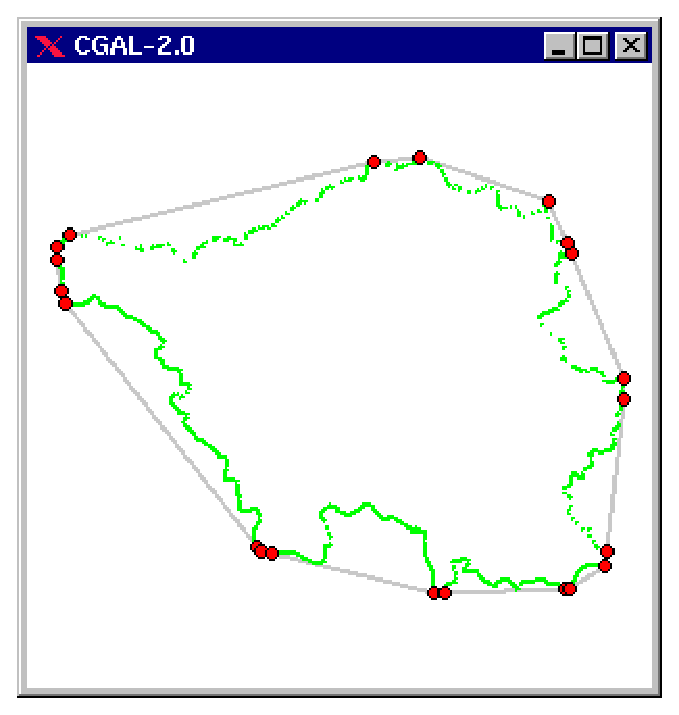
\includegraphics[width=6.5cm]{Convex_hull_2/saarhull}
%\leavevmode\epsfxsize8cm\epsffile{Convex_hull_2/saarhull.eps}
\end{center}
\end{ccTexOnly}

\section{Convex Hull}
\label{sec:convex_hull_2}
\cgal\ provides implementations of several classical algorithms for
computing the counterclockwise sequence of extreme points for a set of 
points in two dimensions (\textit{i.e.}, the counterclockwise sequence 
of points on the convex hull).  The algorithms have different asymptotic
running times and require slightly different sets of geometric primitives. 
Thus you may choose the algorithm that best fits your setting.

Each of the convex hull functions presents the same interface to the
user.  That is, the user provides a pair of iterators, \ccc{first}
and \ccc{beyond}, an output iterator \ccc{result},  and a traits class
\ccc{traits}. The points in the range [\ccc{first}, \ccc{beyond}) define
the input points whose convex hull is to be computed.  The counterclockwise
sequence of extreme points is written to the sequence starting at position
\ccc{result}, and the past-the-end iterator for the resulting set of
points is returned.  The traits classes for the functions specify the types
of the input points and the geometric primitives that are required by
the algorithms. All functions provide an interface in which this
class need not be specified and defaults to types and operations defined
in the kernel in which the input point type is defined.

Given a sequence of $n$ input points with $h$ extreme points,
the function \ccc{convex_hull_2}\ccIndexMainItem[C]{convex_hull_2}
uses either the output-sensitive $O(n h)$ algorithm of Bykat \cite{b-chfsp-78}
(a non-recursive version of the quickhull \cite{bdh-qach-96} algorithm)%
\ccIndexSubitem{convex hull, 2D}{quickhull}
\ccIndexSubitem{convex hull, 2D}{Bykat's algorithm} 
or the algorithm of Akl and Toussaint, which requires $O(n \log n)$ time
in the worst case.  The algorithm chosen depends on the kind of 
iterator used to specify the input points.  These two algorithms are
also available via the functions \ccc{ch_bykat} and \ccc{ch_akl_toussaint},
respectively.  Also available are 
the $O(n \log n)$ Graham-Andrew scan algorithm \cite{a-aeach-79,m-mdscg-84} 
(\ccc{ch_graham_andrew}\ccIndexMainItem[C]{ch_graham_andrew}), 
the $O(n h)$ Jarvis march algorithm \cite{j-ichfs-73}
(\ccc{ch_jarvis}\ccIndexMainItem[C]{ch_jarvis}),
and Eddy's $O(n h)$ algorithm \cite{e-nchap-77}
(\ccc{ch_eddy}\ccIndexMainItem[C]{ch_eddy}), which corresponds to the 
two-dimensional version of the quickhull algorithm.
The linear-time algorithm of Melkman for producing the convex hull of 
simple polygonal chains (or polygons) is available through the function
\ccc{ch_melkman}\ccIndexMainItem[C]{ch_melkman}.%
\ccIndexSubitem{convex hull, 2D}{of polyline or polygon}

\section{Example using Graham-Andrew's Algorithm}

In the following example a convex hull is constructed from point data read 
from standard input using \ccc{Graham_Andrew} algorithm. The resulting convex 
polygon is shown at the standard ouput console. The same results could be 
achieved by substituting the function \ccc{CGAL::ch_graham_andrew} by other 
function like \ccc{CGAL::ch_bykat}.

\ccIncludeExampleCode{Convex_hull_2/ch_example_from_cin_to_cout.cpp}


\section{Extreme Points and Hull Subsequences}
In addition to the functions for producing convex hulls, there are a
number of functions for computing sets and sequences of points related
to the convex hull.  
The functions \ccc{lower_hull_points_2}\ccIndexMainItem[C]{lower_hull_points_2}
and \ccc{upper_hull_points_2}\ccIndexMainItem[C]{upper_hull_points_2}
provide the computation of the counterclockwise 
sequence of extreme points on the lower hull and upper hull,
respectively.  The algorithm used in these functions is
Andrew's variant of Graham's scan algorithm \cite{a-aeach-79,m-mdscg-84},
which has worst-case running time of $O(n \log n)$.

There are also functions available for computing certain subsequences 
of the sequence of extreme points on the convex hull.  The function
\ccc{ch_jarvis_march}\ccIndexMainItem[C]{ch_jarvis_march}
generates the counterclockwise ordered subsequence of
extreme points between a given pair of points and
\ccc{ch_graham_andrew_scan}\ccIndexMainItem[C]{ch_graham_andrew_scan}
computes the sorted sequence of extreme points that are
not left of the line defined by the first and last input points.

Finally, a set of functions 
(\ccc{ch_nswe_point}, \ccc{ch_ns_point}, \ccc{ch_we_point}, \ccc{ch_n_point},
\ccc{ch_s_point}, \ccc{ch_w_point}, \ccc{ch_e_point})
is provided for computing extreme points of a 
2D point set in the coordinate directions.%
\ccIndexSubitem{extreme points, 2D}{in coordinate directions}

\section{Static Convex Hull Construction}
\label{sec:convex_hull_3}

\ccIndexSubitem{convex hull, 3D}{static}
\ccIndexSubitem{convex hull, 3D}{quickhull}

The function 
\ccc{convex_hull_3}\ccIndexMainItem[C]{convex_hull_3} provides an 
implementation of the quickhull algorithm \cite{bdh-qach-96} for three 
dimensions\ccIndexMainItem{quickhull, 3D}.  There are two versions of this
function available, one that can be used when it is known that the output
will be a polyhedron (\textit{i.e.}, there are more than three points and
they are not all collinear) and one that handles all degenerate cases
and returns a \ccc{CGAL::Object}, which may be a point, a segment, a
triangle, or a polyhedron.  Both versions accept a range of input
iterators defining the set of points whose convex hull is to be computed
and a traits class defining the geometric types and predicates used in
computing the hull.

\subsection{Traits Class}

The function \ccc{convex_hull_3} is parameterized by a traits class,
which specifies the types and geometric primitives to be used in the
computation.  The default for this traits class is
\ccc{Convex_hull_traits_3}\ccIndexMainItem[C]{Convex_hull_traits_3}.

\subsection{Convexity Checking}

The function \ccc{is_strongly_convex_3}\ccIndexMainItem[C]{is_strongly_convex_3}
implements the algorithm of Mehlhorn \textit{et al.} \cite{mnssssu-cgpvg-96} 
to determine if the vertices of a given polytope constitute a strongly convex 
point set or not.  This function is used in postcondition testing for
\ccc{convex_hull_3}\ccIndexSubitem[C]{convex_hull_3}{postcondition}.

\subsection{Example}
The following program computes the convex hull of a set of 250 random
points chosen from a sphere of radius 100.  It then determines if the 
resulting hull is a segment or a polyhedron.  

\ccIncludeExampleCode{Convex_hull_3/quickhull_3_ex.C}


\section{Incremental  Convex Hull Construction}
\ccIndexSubitem{convex hull, 3D}{incremental}

The function \ccc{convex_hull_incremental_3} %
\ccIndexMainItem[C]{convex_hull_incremental_3} provides an
interface similar to \ccc{convex_hull_3} for the $d$-dimensional 
incremental construction algorithm \cite{cms-frric-93}.  
implemented by the class \ccc{CGAL::Convex_hull_d<R>} that is specialized 
to three dimensions. This function accepts an iterator range over a set of
input points and returns a polyhedron, but it does not have a traits class
in its interface.  It uses the kernel
class \ccc{Kernel} used in the polyhedron type to define an instance of the 
adapter traits class \ccc{CGAL::Convex_hull_d_traits_3<Kernel>}.

In most cases, the function \ccc{convex_hull_3} will be faster than
\ccc{convex_hull_incremental_3}.  The latter is provided mainly 
for comparison purposes. 

To use the full functionality available with the $d$-dimensional class 
\ccc{CGAL::Convex_hull_d<R>} in three dimensions (\textit{e.g.}, the ability
to insert new points and to query if a point lies in the convex hull or not), 
you can instantiate the class \ccc{CGAL::Convex_hull_d<K>} with the adapter
traits class \ccc{CGAL::Convex_hull_d_traits_3<K>}, as shown in the following
example.

\subsection{Example}

\ccIncludeExampleCode{Convex_hull_3/incremental_hull_3_demo.C}

\section{Dynamic  Convex Hull Construction}
\ccIndexSubitem{convex hull, 3D}{dynamic}

Fully dynamic maintenance of a convex hull can be achieved by using the
class \ccc{CGAL::Delaunay_triangulation_3}.  This class supports insertion
and removal of points (\textit{i.e.}, vertices of the triangulation) and the 
convex hull edges are simply the finite edges of infinite faces.  
The following example illustrates the dynamic construction of a convex hull.
First, random points from a sphere of a certain radius are generated and are
inserted into a triangulation.  Then the number of points of the convex hull 
are obtained by counting the number of triangulation vertices incident to the 
infinite vertex.  Some of the points are removed and then the number of points 
remaining on the hull are determined.  Notice that the vertices incident to the
infinite vertex of the triangulation are on the convex hull but it may be that
not all of them are vertices of the hull.

\subsection{Example}
\ccIncludeExampleCode{Convex_hull_3/dynamic_hull_3_ex.C}



\input{ConvexHull_ref/convex_hull_randomized_incremental_3.tex}
% +------------------------------------------------------------------------+
% | Reference manual page: ConvexHullPolyhedronFacet_3.tex
% +------------------------------------------------------------------------+
% | 17.03.1999   Lutz Kettner
% | Package: Polyhedron
% | 
\RCSdef{\RCSFacetRev}{$Revision$}
\RCSdefDate{\RCSFacetDate}{$Date$}
% +------------------------------------------------------------------------+

\ccRefPageBegin

%%RefPage: end of header, begin of main body
% +------------------------------------------------------------------------+


\begin{ccRefConcept}{ConvexHullPolyhedronFacet_3}

\ccDefinition
  
The requirements of the facet type of a polyhedron to be built by the
function \ccc{convex_hull_3}.

\ccHasModels
\ccRefIdfierPage{CGAL::Polyhedron<Traits>::Facet}

\ccTypes
\ccNestedType{Plane}{plane equation type stored in facets.}

\ccNestedType{Halfedge_handle}{handle to halfedge.}

\ccNestedType{Halfedge_around_facet_circulator}{circulator of
  halfedges around a facet.}

\ccCreation
\ccCreationVariable{f}

\ccConstructor{Facet();}{default constructor.}

\ccOperations
\ccTagFullDeclarations
         
\ccMethod{Plane&       plane();}{}
\ccGlue
\ccMethod{const Plane& plane() const;}{plane equation.}

%\ccHeading{Operations available if \ccc{Supports_facet_halfedge} $\equiv$ 
%           \ccc{CGAL::Tag_true}}

\ccMethod{Halfedge_handle       halfedge();}%
{ an incident halfedge that points to \ccVar.}
\ccGlue

\ccMethod{Halfedge_around_facet_circulator       facet_begin();}
{circulator of halfedges around the facet (counterclockwise).}

\ccSeeAlso
\ccRefIdfierPage{CGAL::Polyhedron_3<Traits>} \\
\ccRefConceptPage{ConvexHullPolyhedronVertex_3} \\
\ccRefConceptPage{ConvexHullPolyhedronHalfedge_3} 

\ccTagDefaults
\end{ccRefConcept}

% +------------------------------------------------------------------------+
%%RefPage: end of main body, begin of footer
\ccRefPageEnd
% EOF
% +------------------------------------------------------------------------+

% +------------------------------------------------------------------------+
% | Reference manual page: ConvexHullPolyhedronHalfedge_3.tex
% +------------------------------------------------------------------------+
% | 17.03.1999   Lutz Kettner
% | Package: Polyhedron
% | 
\RCSdef{\RCSHalfedgeRev}{$Revision$}
\RCSdefDate{\RCSHalfedgeDate}{$Date$}
% +------------------------------------------------------------------------+

\ccRefPageBegin

%%RefPage: end of header, begin of main body
% +------------------------------------------------------------------------+


\begin{ccRefConcept}{ConvexHullPolyhedronHalfedge_3}

\ccDefinition

The requirements of the halfedge type required for the polyhedron built
by the function \ccc{convex_hull_3}.
  
\ccHasModels
\ccRefIdfierPage{CGAL::Polyhedron_3<Traits>::Halfedge}

\ccCreation
\ccCreationVariable{h}

\ccConstructor{Halfedge();}{default constructor.}

\ccTagFullDeclarations
\ccOperations

\ccMethod{Halfedge_handle opposite();}{the opposite halfedge.}

\ccMethod{Halfedge_handle next();}
    {the next halfedge around the facet.}

\ccMethod{Halfedge_handle prev();}
    {the previous halfedge around the facet.}

\ccMethod{bool             is_border() const;}
    {is true if \ccVar\ is a border halfedge.}


\ccMethod{Halfedge_around_facet_circulator       facet_begin();}
    {circulator of halfedges around the facet (counterclockwise).}


\ccMethod{Vertex_handle       vertex();}{the incident vertex of \ccVar.}

\ccMethod{Facet_handle       facet();}
    {the incident facet of \ccVar.  If \ccVar\ is a border halfedge 
      the result is default construction of the handle.}


\ccSeeAlso

\ccRefIdfierPage{CGAL::Polyhedron_3<Traits>} \\
\ccRefConceptPage{ConvexHullPolyhedronVertex_3} \\
\ccRefConceptPage{ConvexHullPolyhedronFacet_3} 

\ccTagDefaults
\end{ccRefConcept}

% +------------------------------------------------------------------------+
%%RefPage: end of main body, begin of footer
\ccRefPageEnd
% EOF
% +------------------------------------------------------------------------+

% +------------------------------------------------------------------------+
% | Reference manual page: ConvexHullPolyhedronVertex_3.tex
% +------------------------------------------------------------------------+
% | 17.03.1999   Lutz Kettner
% | Package: Polyhedron
% | 
\RCSdef{\RCSVertexRev}{$Id$}
\RCSdefDate{\RCSVertexDate}{$Date$}
% +------------------------------------------------------------------------+

\ccRefPageBegin

%%RefPage: end of header, begin of main body
% +------------------------------------------------------------------------+


\begin{ccRefConcept}{ConvexHullPolyhedronVertex_3}

\ccDefinition

The requirements of the vertex type of the polyhedron to be built by the
function \ccc{convex_hull_3}.  

\ccHasModels

\ccRefIdfierPage{CGAL::Polyhedron_3<Traits>::Vertex}.

\ccCreation
\ccCreationVariable{v}

\ccConstructor{Vertex();}{default constructor.}
%\ccGlue
%\ccConstructor{Vertex( const Point& p);}{vertex initialized with a point.}

\ccOperations

\ccTagFullDeclarations
\ccMethod{Point&       point();}{}
\ccGlue
\ccMethod{const Point& point() const;}{the point.}

\ccSeeAlso

\ccRefIdfierPage{CGAL::Polyhedron_3<Traits>} \\
\ccRefConceptPage{ConvexHullPolyhedronFacet_3} \\
\ccRefConceptPage{ConvexHullPolyhedronHalfedge_3} 

\ccTagDefaults
\end{ccRefConcept}

% +------------------------------------------------------------------------+
%%RefPage: end of main body, begin of footer
\ccRefPageEnd
% EOF
% +------------------------------------------------------------------------+


\begin{ccRefConcept}{ConvexHullPolyhedron_3}

\ccDefinition
The requirements of the polyhedron type to be built by the
function \ccc{convex_hull_3}.

\ccHasModels

\ccRefIdfierPage{CGAL::Polyhedron_3<Traits>}

\ccTypes
\ccAutoIndexingOff
\ccNestedType{Point_3}{ type of point stored in a vertex }
\ccGlue
\ccNestedType{Vertex}{ a model of \ccc{ConvexHullPolyhedronVertex_3}}
\ccGlue
\ccNestedType{Halfedge}{ a model of \ccc{ConvexHullPolyhedronHalfedge_3}}
\ccGlue
\ccNestedType{Facet}{ a model of \ccc{ConvexHullPolyhedronFacet_3} }
\ccGlue
\ccNestedType{Halfedge_data_structure}{halfedge data structure}
\ccGlue
\ccNestedType{Halfedge_handle}{handle to halfedge}
\ccGlue
\ccNestedType{Halfedge_iterator}{iterator for halfedge}
\ccGlue
\ccNestedType{Facet_handle}{handle to facet}
\ccGlue
\ccNestedType{Facet_iterator}{iterator for facet}

\ccCreation
\ccCreationVariable{p}

Only a default constructor is required.

\ccConstructor{ConvexHullPolyhedron_3();}{}

\ccOperations

\ccAutoIndexingOff
\ccMethod{Facet_iterator facets_begin();}%
{iterator over all facets (excluding holes).}

\ccMethod{Facet_iterator facets_end();}{past-the-end iterator.}

\ccMethod{Halfedge_iterator P.halfedges_begin();}{ iterator over all halfedges.}
\ccMethod{Halfedge_iterator P.halfedges_end();}{past-the-end iterator.}

\ccMethod{
Halfedge_handle make_tetrahedron(Point_3 p1, Point_3 p2, Point_3 p3, Point_3 p4);
}{
adds a new tetrahedron to the polyhedral surface with its
vertices initialized with \ccc{p1}, \ccc{p2}, \ccc{p3} and \ccc{p4}. 
Returns that halfedge
of the tetrahedron which incident vertex is initialized with \ccc{p1}, the
incident vertex of the next halfedge with \ccc{p2}, and the vertex
thereafter with \ccc{p3}. The remaining fourth vertex is initialized with
\ccc{p4}.
}

\ccMethod{void erase_facet(Halfedge_handle h);}%
{removes the incident facet of \ccc{h} 
and changes all halfedges incident to the facet into border edges or removes 
them from the polyhedral surface if they were already border edges.}


\ccMethod{
Halfedge_handle 
add_vertex_and_facet_to_border(Halfedge_handle h, Halfedge_handle g);
}{
creates a new facet within the hole incident to \ccc{h} and \ccc{g} by
connecting the tip of \ccc{g} with the tip of \ccc{h} with two new halfedges
and a new vertex and filling this separated part of the hole with
a new facet, such that the new facet is incident to \ccc{g}. Returns the
halfedge of the new edge that is incident to the new facet and
the new vertex.
}

\ccMethod{
Halfedge_handle
add_facet_to_border(Halfedge_handle h, Halfedge_handle g);}%
{
creates a new facet within the hole incident to \ccc{h} and \ccc{g} by
connecting the tip of \ccc{g} with the tip of \ccc{h} with a new halfedge and
filling this separated part of the hole with a new facet, such that
the new facet is incident to \ccc{g}. Returns the halfedge of the new
edge that is incident to the new facet.
}

\ccMethod{Halfedge_handle fill_hole(Halfedge_handle h);}{
fills a hole with a newly created facet. Makes all border
halfedges of the hole denoted by h incident to the new facet.
Returns \ccc{h}.
}

\ccMethod{void delegate(Modifier_base<Halfedge_data_structure>& m);}%
{
calls the \ccc{operator()} of the modifier \ccc{m}. See \ccc{Modifier_base}
for a description of modifier design and its usage.
}
\ccAutoIndexingOn


\end{ccRefConcept}

% +------------------------------------------------------------------------+
% | Reference manual page: ConvexHullTraits_2.tex
% +------------------------------------------------------------------------+
% | 14.05.2001   Susan Hert and Stefan Schirra
% | Package: Convex_hull_2
% | 
% +------------------------------------------------------------------------+


\begin{ccRefConcept}{ConvexHullTraits_2}
\ccIndexTraitsClassRequirements[p]{convex hull, 2D}
\ccIndexTraitsClassRequirements[p]{extreme points, 2D}

\ccDefinition
  
All convex hull and extreme point algorithms provided in \cgal\ are
parameterized with a traits class \ccStyle{Traits}, which defines the
primitives (objects and predicates) that the convex hull algorithms use.
\ccRefName\ defines the complete set of primitives required in these
functions.  The specific subset of these primitives required by each function
is specified with each function.

\ccTypes
\ccAutoIndexingOff
\ccSetTwoColumns{ConvexHullTraits_2::Left_of_line_2}{}

\ccNestedType{Point_2}%
       {The point type on which the convex hull functions operate.}

\ccNestedType{Less_xy_2}%
       {Binary predicate object type comparing \ccc{Point_2}s
        lexicographically.  Must provide 
        \ccc{bool operator()(Point_2 p, Point_2 q)} where \ccc{true}
        is returned iff $p <_{xy} q$.
        We have $p<_{xy}q$, iff $p_x < q_x$ or $p_x = q_x$ and $p_y < q_y$,
        where $p_x$ and $p_y$ denote $x$ and $y$ coordinate of point $p$,
        respectively.
       }

\ccNestedType{Less_yx_2}%
       {Same as \ccc{Less_xy_2} with the roles of $x$ and $y$ interchanged.}

\ccNestedType{Leftturn_2}%
       {Predicate object type that must provide
        \ccc{bool operator()(Point_2 p,Point_2 q,Point_2 r)}, which
        returns \ccc{true} iff \ccc{r} lies to the left of the
        oriented line through \ccc{p} and \ccc{q}.}

\ccNestedType{Left_of_line_2}%
       {Unary predicate object type that
        must provide a constructor taking two \ccc{Point_2}s, $p$ and
        $q$, and \ccc{bool operator()(Point_2 r)}, which returns \ccc{true} iff
        $r$ lies to the left of the directed line through $p$ and $q$.}

\ccNestedType{Less_signed_distance_to_line_2}%
       {Binary predicate object type that must provide a constructor taking
        two \ccc{Point_2}s, $p$ and $q$, and
        \ccc{bool operator()(Point_2 r,Point_2 s)}, which returns \ccc{true} iff
        the signed distance from $r$ to the line $l_{pq}$ through $p$ and $q$
        is smaller than the distance from $s$ to $l_{pq}$. It is used to
        compute the point right of a line with maximum unsigned distance to
        the line. The binary predicate must provide a total order compatible
        with convexity, {\it i.e.}, for any line segment $s$ one of the 
        endpoints 
        of $s$ is the smallest point among the points on $s$, with respect to
        the order given by \ccc{Less_signed_distance_to_line_2}.}

\ccNestedType{Less_rotate_ccw_2}%
       {Binary predicate object type that must provide a constructor taking a
        \ccc{Point_2}, $e$, and \ccc{bool operator()(Point_2 p,Point_2 q)},
        where \ccc{true} is returned iff a tangent at $e$ to the point set
        $\{e,p,q\}$ hits $p$ before $q$ when rotated counterclockwise around 
        $e$.
        Ties are broken such that the point with larger distance to $e$
        is smaller!}


\ccCreation
\ccCreationVariable{traits}  %% choose variable name

Only a copy constructor is required.

\ccConstructor{ConvexHullTraits_2(ConvexHullTraits_2& t);}{}

\ccOperations

The following member functions to create instances of the above predicate
object types must exist. 

\setlength\parskip{0mm}
\ccMemberFunction{Less_xy_2 less_xy_2_object(); }{}
\ccGlue
\ccMemberFunction{Less_yx_2 less_yx_2_object(); }{}
\ccGlue
\ccMemberFunction{Left_of_line_2 left_of_line_2_object( const Point_2& p, const
Point_2& q) ; }{}
\ccGlue
\ccMemberFunction{Less_signed_distance_to_line_2 less_signed_distance_to_line_2_object( const Point_2& p, const Point_2& q); }{}
\ccGlue
\ccMemberFunction{Less_rotate_ccw_2 less_rotate_ccw_2_object( const Point_2& p )
; }{}
\ccGlue
\ccMemberFunction{Leftturn_2 leftturn_2_object(); }{}


\ccParDims
\ccHasModels

\ccRefIdfierPage{CGAL::Convex_hull_constructive_traits_2<R>} \\
\ccRefIdfierPage{CGAL::Convex_hull_leda_traits_2} \\
\ccRefIdfierPage{CGAL::Convex_hull_projective_xy_traits_2<Point_3>} \\
\ccRefIdfierPage{CGAL::Convex_hull_projective_xz_traits_2<Point_3>} \\
\ccRefIdfierPage{CGAL::Convex_hull_projective_yz_traits_2<Point_3>} \\
\ccRefIdfierPage{CGAL::Convex_hull_rat_leda_traits_2} \\
\ccRefIdfierPage{CGAL::Convex_hull_traits_2<R>} \\
\ccAutoIndexingOn

\ccSeeAlso

\ccRefConceptPage{IsStronglyConvexTraits_3}

\ccParDims
\end{ccRefConcept}

% +------------------------------------------------------------------------+
%%RefPage: end of main body, begin of footer
% EOF
% +------------------------------------------------------------------------+


\begin{ccRefConcept}{ConvexHullTraits_3}

\ccDefinition
Requirements of the traits class to be used with the function
\ccc{convex_hull_3}. 

\ccTypes
\ccAutoIndexingOff
\ccNestedType{Point_3}{The point type on which the convex hull algorithm operates}
\ccGlue
\ccNestedType{Plane_3}{a 3D plane}
\ccGlue
\ccNestedType{Segment_3}{a 3D segment}
\ccGlue
\ccNestedType{Triangle_3}{a 3D triangle}
\ccGlue
\ccNestedType{Vector_3}{a 3D vector}

\ccNestedType{Construct_plane_3}{Function object type that provides
\ccc{Plane_3 operator()(Point_3 p, Point_3 q, Point_2 r)}, which constructs
and returns a plane passing through \ccc{p}, \ccc{q}, and \ccc{r} and oriented
in a positive sense when seen from the positive side of the plane.}

\ccNestedType{Construct_segment_3}{Function object type that provides
\ccc{Segment_3 operator()(Point_3 p, Point_3 q)}, which constructs and
returns the segment with source \ccc{p} and target \ccc{q}.}

\ccNestedType{Construct_triangle_3}{Function object type that provides
\ccc{Triangle_3 operator()(Point_3 p, Point_3 q, Point_3 r)}, which 
constructs and returns the triangle with vertices \ccc{p}, \ccc{q}, and
\ccc{r}}

\ccNestedType{Construct_vector_3}{Function object type that provides
\ccc{Vector_3 operator()(Point_3 p, Point_3 q)}, which constructs and
returns the vector \ccc{q}-\ccc{p}}

\ccNestedType{Collinear_3}{Predicate object type that provides
\ccc{bool operator()(Point_3 p, Point_3 q, Point_3 r)}, which determines
if points \ccc{p}, \ccc{q} and \ccc{r} are collinear or not}

\ccNestedType{Coplanar_3}{Predicate object type that provides
\ccc{bool operator()(Point_3 p, Point_3 q, Point_3 r, Point_3 s)}, which 
determines if points \ccc{p}, \ccc{q}, \ccc{r}, and \ccc{s} are coplanar
or not}

\ccNestedType{Has_on_positive_side_3}{Predicate object type that provides
\ccc{bool operator()(Plane_3 h, Point_3 q)}, which determines of the point
\ccc{q} is on the positive side of the halfspace \ccc{h}}

\ccNestedType{Less_distance_to_point_3}{Predicate object type that provides
a constructor taking a single \ccc{Point_3} object and
\ccc{bool operator()(Point_3 q, Point_3 r)}, which returns true iff the
distance from \ccc{q} to \ccc{p} is smaller than the distance from
\ccc{r} to \ccc{p}, where \ccc{p} is the point passed to the object
at construction.}

\ccNestedType{Less_signed_distance_to_plane_3}{Predicate object type that
provides \ccc{bool operator()(Plane_3 p, Point_3 q, Point_3 r)}, which 
returns true iff the signed distance from \ccc{q} to \ccc{p} is smaller
than the signed distance from \ccc{r} to \ccc{p}}

To handle the degenerate case when all points are coplanar, the following
three types that are default-constructable are necessary:

\ccNestedType{Traits_xy}{A model of ConvexHullTraits\_2 for points projected
                         into the $xy$-plane}
\ccNestedType{Traits_xz}{A model of ConvexHullTraits\_2 for points projected
                         into the $xz$-plane}
\ccNestedType{Traits_yz}{A model of ConvexHullTraits\_2 for points projected
                         into the $yz$-plane}

These types need not be provided when it is known that the points are
not all coplanar.

\ccCreation
\ccCreationVariable{traits}

Only a copy constructor is required.

\ccConstructor{ConvexHullTraits_3(ConvexHullTraits_3& ch);}{}

\ccOperations

For each of the above function and predicate object types,
\ccc{Func_obj_type}, a function must exist with the name 
\ccc{func_obj_type_object} that creates an instance of the function or 
predicate object type.  For example:

\ccMethod{Construct_plane_3 construct_plane_3_object();}{}

\ccAutoIndexingOn

\ccHasModels
\ccRefIdfierPage{CGAL::Convex_hull_traits_3<R>}

%\ccSeeAlso

\end{ccRefConcept}

% +------------------------------------------------------------------------+
% | Reference manual page: Convex_hull_constructive_traits_2.tex
% +------------------------------------------------------------------------+
% | 14.05.2001   Susan Hert and Stefan Schirra
% | Package: Convex_hull_2
% | 
% +------------------------------------------------------------------------+

\ccAutoIndexingOff
\begin{ccRefClass}{Convex_hull_constructive_traits_2<R>}
\ccAutoIndexingOn
\ccIndexTraitsClassBegin{Convex_hull_constructive_traits_2}{}{convex hull, 2D}

\ccDefinition
  
The class \ccRefName\ serves as a traits class for all the two-dimensional
convex hull and extreme point calculation function. Unlike the class
\ccc{CGAL::Convex_hull_traits_2<R>}, this class makes use of previously
computed results to avoid redundancy.  For example,
in the sidedness tests, lines (of type \ccc{R::Line_2}) are constructed,
which is equivalent to the precomputation of subdeterminants of
the orientation-determinant for three points.

\ccInclude{CGAL/convex_hull_constructive_traits_2.h}

\ccIsModel

\ccRefConceptPage{ConvexHullTraits_2}%
\ccIndexSubitem[c]{ConvexHullTraits_2}{model} \\

\ccTypes
\ccAutoIndexingOff
\ccSetThreeColumns{typedef R::Less_signed_distance_to_line_2 }{Less_signed_distance_to_line_2}{}
\ccThreeToTwo

\ccTypedef{typedef R::Point_2                        Point_2;}{}
\ccGlue
\ccTypedef{typedef R::Less_xy                        Less_xy_2;}{}
\ccGlue
\ccTypedef{typedef R::Less_yx                        Less_yx_2;}{}
\ccGlue
\ccTypedef{typedef CGAL::r_Less_dist_to_line<R>
                                      Less_signed_distance_to_line_2;}{}
\ccGlue
\ccTypedef{typedef R::Less_rotate_ccw                Less_rotate_ccw_2;}{}
\ccGlue
\ccTypedef{typedef R::Leftturn_2                     Leftturn_2;}{}


\ccCreation
\ccCreationVariable{traits}  %% choose variable name

\ccConstructor{Convex_hull_constructive_traits_2();}{default constructor.}

\ccOperations
\ccAutoIndexingOff
\ccMemberFunction{Less_xy_2 less_xy_2_object(); }{}
\ccGlue
\ccMemberFunction{Less_yx_2 less_yx_2_object(); }{}
\ccGlue
\ccMemberFunction{Less_signed_distance_to_line_2 
                  less_signed_distance_to_line_2_object();}{}
\ccGlue
\ccMemberFunction{Less_rotate_ccw_2 
                  less_rotate_ccw_2_object(); }{}
\ccGlue
\ccMemberFunction{Leftturn_2 leftturn_2_object(); }{}
\ccAutoIndexingOn


\ccSeeAlso

\ccRefIdfierPage{CGAL::Convex_hull_leda_traits_2}  \\
\ccRefIdfierPage{CGAL::Convex_hull_rat_leda_traits_2}  \\
\ccRefIdfierPage{CGAL::Convex_hull_projective_xy_traits_2<Point_3>} \\
\ccRefIdfierPage{CGAL::Convex_hull_projective_xz_traits_2<Point_3>} \\
\ccRefIdfierPage{CGAL::Convex_hull_projective_yz_traits_2<Point_3>}  \\
\ccRefIdfierPage{CGAL::Convex_hull_traits_2<R>}  

\ccIndexTraitsClassEnd
\ccAutoIndexingOff
\end{ccRefClass}
\ccAutoIndexingOn

% EOF

% begin cgal manual page

\begin{ccRefClass}{Convex_hull_d<R>}\ccCreationVariable{C}

\ccDefinition

An instance \ccc{C} of type \ccc{Convex_hull_d<R>} is the convex
hull of a multi-set \ccc{S} of points in $d$-dimensional space. We call
\ccc{S} the underlying point set and $d$ or \ccc{dim} the dimension of the
underlying space. We use \ccc{dcur} to denote the affine dimension of \ccc{S}.
The data type supports incremental construction of hulls.

The closure of the hull is maintained as a simplicial complex, i.e.,
as a collection of simplices. The intersection of any two is a face of
both\footnote{The empty set if a facet of every simplex.}. In the
sequel we reserve the word simplex for the simplices of dimension
\ccc{dcur}. For each simplex there is a handle of type \ccc{Simplex_handlex}
and for each vertex there is a handle of type \ccc{Vertex_handle}.  Each
simplex has $1 + \ccc{dcur}$ vertices indexed from $0$ to \ccc{dcur}; for a
simplex $s$ and an index $i$, \ccc{C.vertex(s,i)} returns the $i$-th
vertex of $s$. For any simplex $s$ and any index $i$ of $s$ there may
or may not be a simplex $t$ opposite to the $i$-th vertex of $s$.  The
function \ccc{C.opposite_simplex(s,i)} returns $t$ if it exists and
returns \ccc{Simplex_handle()} (the undefined handle) otherwise. If $t$
exists then $s$ and $t$ share \ccc{dcur} vertices, namely all but the
vertex with index $i$ of $s$ and the vertex with index
\ccc{C.index_of_vertex_in_opposite_simplex(s,i)} of $t$. Assume that $t$
exists and let \ccc{j = C.index_of_vertex_in_opposite_simplex(s,i)}.  Then
$s =$ \ccc{C.opposite_simplex(t,j)} and $i =$
\ccc{C.index_of_vertex_in_opposite_simplex(t,j)}.

The boundary of the hull is also a simplicial complex. All simplices
in this complex have dimension $\ccc{dcur} - 1$.  For each boundary simplex
there is a handle of type \ccc{Facet_handle}.  Each facet has \ccc{dcur} vertices
indexed from $0$ to $\ccc{dcur} - 1$. If \ccc{dcur > 1} then for each facet $f$
and each index $i$, $0 \le i < \ccc{dcur}$, there is a facet $g$ opposite
to the $i$-th vertex of $f$.  The function \ccc{C.opposite_facet(f,i)}
returns $g$.  Two neighboring facets $f$ and $g$ share \ccc{dcur - 1}
vertices, namely all but the vertex with index $i$ of $f$ and the
vertex with index \ccc{C.index_of_vertex_in_opposite_facet(f,i)} of $g$.
Let \ccc{j = C.index_of_vertex_in_opposite_facet(f,i)}. Then 
\ccc{f = C.opposite_facet(g,j)} and 
\ccc{i = C.index_of_vertex_in_opposite_facet(g,j)}. 



\ccSetOneOfTwoColumns{6.5cm}

\ccTypes

\ccNestedType{R}{the representation class. 
}

\ccNestedType{Point_d}{the point type. 
}

\ccNestedType{Hyperplane_d}{the hyperplane type. 
}

\ccNestedType{Simplex_handle}{handle for simplices. 
}

\ccNestedType{Facet_handle}{handle for facets. 
}

\ccNestedType{Vertex_handle}{handle for vertices. 
}

\ccNestedType{Simplex_iterator}{iterator for simplices. 
}

\ccNestedType{Vertex_iterator}{iterator for vertices. 
}

\ccNestedType{Point_const_iterator}{const iterator for points. 
}

\ccSetOneOfTwoColumns{3cm}

\ccCreation

\ccConstructor{Convex_hull_d<R>(int d, R Kernel = R())}{creates an instance \ccc{C} of type \ccc{Convex_hull_d}. The
dimension of the underlying space is $d$ and \ccc{S} is initialized to the
empty point set. The traits class \ccc{R} specifies the models of
all types and the implementations of all geometric primitives used by
the convex hull class. The default model is one of the $d$-dimensional
representation classes (e.g., \ccc{Homogeneous_d}). 
}

The data type \ccc{Convex_hull_d} offers neither copy constructor nor
assignment operator. 

\ccHeading{Requirements}

\ccc{R} is a model of the concept \ccc{ConvexHullTraits_d}
  \ccIndexMainItem[c]{ConvexHullTraits_d}.                    

\ccSetOneOfTwoColumns{3cm}

\ccOperations

All operations below that take a point \ccc{x} as argument have the
common precondition that \ccc{x} is a point of ambient space.



\ccMethod{int dimension() ;}{returns the dimension of ambient space }

\ccMethod{int current_dimension() ;}{%
returns the affine dimension \ccc{dcur} of $S$. }

\ccMethod{Point_d  associated_point(Vertex_handle v) ;}{%
returns the point associated with vertex $v$.}

\ccMethod{Vertex_handle  vertex_of_simplex(Simplex_handle s, int i) ;}{returns the vertex corresponding to the $i$-th vertex of $s$.\\
\ccPrecond $0 \leq i \leq \ccc{dcur}$.  
}

\ccMethod{Point_d  point_of_simplex(Simplex_handle s,int i) ;}{same as \ccc{C.associated_point(C.vertex_of_simplex(s,i))}.  
}

\ccMethod{Simplex_handle opposite_simplex(Simplex_handle s,int i) ;}{returns the simplex opposite to the $i$-th vertex of $s$
(\ccc{Simplex_handle()} if there is no such simplex). 
\ccPrecond $0 \leq i \leq \ccc{dcur}$.  
}

\ccMethod{int  index_of_vertex_in_opposite_simplex(Simplex_handle s,int i) ;}{returns the index of the vertex opposite to the $i$-th vertex
of $s$. \ccPrecond $0 \leq i \leq \ccc{dcur}$ and there is a
simplex opposite to the $i$-th vertex of $s$.  
}

\ccMethod{Simplex_handle  simplex(Vertex_handle v) ;}{returns a simplex of which $v$ is a node. Note that this
simplex is not unique.  
}

\ccMethod{int index(Vertex_handle v) ;}{returns the index of $v$ in \ccc{simplex(v)}. 
}

\ccMethod{Vertex_handle  vertex_of_facet(Facet_handle f, int i) ;}{returns the vertex corresponding to the $i$-th vertex of $f$.
\ccPrecond $0 \leq i < \ccc{dcur}$.  
}

\ccMethod{Point_d point_of_facet(Facet_handle f, int i) ;}{same as \ccc{C.associated_point(C.vertex_of_facet(f,i))}. 
}

\ccMethod{Facet_handle opposite_facet(Facet_handle f, int i) ;}{returns the facet opposite to the $i$-th vertex of $f$
(\ccc{Facet_handle()} if there is no such facet). \ccPrecond $0 \leq i <
\ccc{dcur}$ and \ccc{dcur > 1}.  
}

\ccMethod{int index_of_vertex_in_opposite_facet(Facet_handle f, int i) ;}{returns the index of the vertex opposite to the $i$-th vertex of 
$f$. \ccPrecond $0 \leq i < \ccc{dcur}$ and \ccc{dcur > 1}. 
}

\ccMethod{Hyperplane_d hyperplane_supporting(Facet_handle f) ;}{returns a hyperplane supporting facet \ccc{f}. The hyperplane is
oriented such that the interior of \ccc{C} is on the negative
side of it. \ccPrecond \ccc{f} is a facet of \ccc{C} and \ccc{dcur > 1}. 
}

\ccMethod{Vertex_handle insert(const Point_d& x);}{adds point \ccc{x} to the underlying set of points.  If $x$ is
equal to (the point associated with) a vertex of the current hull this
vertex is returned and its associated point is changed to $x$. If $x$
lies outside the current hull, a new vertex \ccc{v} with associated point
$x$ is added to the hull and returned. In all other cases, i.e., if
$x$ lies in the interior of the hull or on the boundary but not on a
vertex, the current hull is not changed and \ccc{Vertex_handle()} is 
returned. If \ccc{CGAL_CHECK_EXPENSIVE} is defined then the validity
check \ccc{is_valid(true)} is executed as a post condition. 
}

\ccMethod{template <typename Forward_iterator>
void insert(Forward_iterator first, Forward_iterator last) ;}{adds \ccc{S = set [first,last)} to the underlying set of
points. If any point \ccc{S[i]} is equal to (the point associated with) a
vertex of the current hull its associated point is changed to \ccc{S[i]}. 
}

\ccMethod{bool is_dimension_jump(const Point_d& x) ;}{returns true if $x$ is not contained in the affine hull of \ccc{S}. 
}

\ccMethod{std::list<Facet_handle>  facets_visible_from(const Point_d& x);}{returns the list of all facets that are visible from \ccc{x}.\\
\ccPrecond \ccc{x} is contained in the affine hull of \ccc{S}. 
}

\ccMethod{Bounded_side bounded_side(const Point_d& x);}{returns \ccc{ON_BOUNDED_SIDE} (\ccc{ON_BOUNDARY},\ccc{ON_UNBOUNDED_SIDE}) 
if \ccc{x} is contained in the interior (lies on the boundary, is contained 
in the exterior) of \ccc{C}. \ccPrecond \ccc{x} is contained in the affine 
hull of \ccc{S}. 
}

\ccMethod{void clear(int d) ;}{reinitializes \ccc{C} to an empty hull in $d$-dimensional space. 
}

\ccMethod{int number_of_vertices() ;}{returns the number of vertices of \ccc{C}. 
}

\ccMethod{int number_of_facets() ;}{returns the number of facets of \ccc{C}. 
}

\ccMethod{int number_of_simplices() ;}{returns the number of bounded simplices of \ccc{C}. 
}

\ccMethod{void print_statistics() ;}{gives information about the size of the current hull and the
number of visibility tests performed. 
}

\ccMethod{bool is_valid(bool throw_exceptions = false) ;}{checks the validity of the data structure.
If \ccc{throw_exceptions == thrue} then the program throws
the following exceptions to inform about the problem.\\
\ccc{chull_has_center_on_wrong_side_of_hull_facet} the hyperplane
supporting a facet has the wrong orientation.\\
\ccc{chull_has_local_non_convexity} a ridge is locally non convex.\\
\ccc{chull_has_double_coverage} the hull has a winding number larger
than 1.
}

\ccHeading{Lists and Iterators}

\ccMethod{Point_const_iterator points_begin() ;}{returns the start iterator for points in \ccc{C}. 
}

\ccMethod{Point_const_iterator points_end() ;}{returns the past the end iterator for points in \ccc{C}. 
}

\ccMethod{Vertex_iterator vertices_begin() ;}{the first vertex of \ccc{C}. 
}

\ccMethod{Vertex_iterator vertices_end()   ;}{the past the end iterator for vertices. 
}

\ccMethod{Simplex_iterator simplices_begin() ;}{the first simplex of \ccc{C}. 
}

\ccMethod{Simplex_iterator simplices_end()   ;}{the past the end iterator for simplices. 
}


\ccMethod{template <typename Visitor>
void visit_all_facets(const Visitor& V) ;}{each facet of \ccc{C} is visited by the visitor object \ccc{V}.
\ccc{V} has to have a function call operator:\\
\ccc{void operator()(Facet_handle) const} 
}

\ccMethod{const std::list<Point_d>& all_points() ;}{returns a list of all points in \ccc{C}. 
}

\ccMethod{std::list<Vertex_handle> all_vertices() ;}{returns a list of all vertices of \ccc{C}
(also interior ones). 
}

\ccMethod{std::list<Simplex_handle> all_simplices() ;}{returns a list of all simplices in \ccc{C}. 
}

\ccMethod{std::list<Facet_handle>  all_facets()  ;}{returns a list of all facets of \ccc{C}. 
}


\ccHeading{Iteration Statements}

{\bf forall\_ch\_simplices}($s,C$)       
$\{$ ``the simplices of $C$ are successively assigned to $s$'' $\}$

{\bf forall\_ch\_vertices}($v,C$)       
$\{$ ``the vertices of $C$ are successively assigned to $v$'' $\}$

 



\ccImplementation

The implementation of type \ccc{Convex_hull_d} is based on
\cite{cms:fourresults-93} and \cite{BMS:degeneracy-94}.  The details
of the implementation can be found in the implementation document
available at the download site of this package.

The time and space requirements are input dependent.  Let $C_1$, $C_2$,
$C_3$, \ldots be the sequence of hulls constructed and for a point $x$
let $k_i$ be the number of facets of $C_i$ that are visible from $x$
and that are not already facets of $C_{i-1}$. Then the time for
inserting $x$ is $O(\ccc{dim} \sum_i k_i)$ and the number of new simplices
constructed during the insertion of $x$ is the number of facets of the
hull which were not already facets of the hull before the insertion.

The data type \ccc{Convex_hull_d} is derived from
\ccc{Regular_complex_d}. The space requirement of regular complexes is
essentially $12(\ccc{dim} +2)$ bytes times the number of simplices
plus the space for the points. \ccc{Convex_hull_d} needs an additional
$8 + (4 + x)\ccc{dim}$ bytes per simplex where $x$ is the space
requirement of the underlying number type and an additional $12$ bytes
per point. The total is therefore $(16 + x)\ccc{dim} + 32$ bytes times
the number of simplices plus $28 + x \cdot \ccc{dim}$ bytes times the
number of points.

\ccHeading{Low Dimensional Conversion Routine}
include \ccc{<CGAL/Convex_hull_d_to_polyhedron_3.h>}

\ccFunction{template <class R, class T, class HDS>
void convex_hull_d_to_polyhedron_3(   const Convex_hull_d<R>& C, Polyhedron_3<T,HDS>& P) ;}{converts the convex hull \ccc{C} to polyedral surface stored in 
   \ccc{P}.\\ \ccPrecond \ccc{dim == 3} and \ccc{dcur == 3}.  
}

\ccHeading{Low Dimensional Output Routines}
include \ccc{<CGAL/IO/Convex_hull_d_window_stream.h>}

\ccFunction{template <class R>
void d2_show(const Convex_hull_d<R>& C, CGAL::Window_stream& W);}{draws the convex hull \ccc{C} in window \ccc{W}.\\
\ccPrecond \ccc{dim == 2}.  
}

\ccFunction{template <class R>
void d3_surface_map(const Convex_hull_d<R>& C, GRAPH< typename Convex_hull_d<R>::Point_d ,int>& G);}{constructs the representation of the surface of \ccc{C} as a 
bidirected LEDA graph \ccc{G}.\\ \ccPrecond \ccc{dim == 3}. 
}

\end{ccRefClass}



% +------------------------------------------------------------------------+
% | Reference manual page: Convex_hull_traits_d.tex
% +------------------------------------------------------------------------+
% | 17.05.2001   Michael Seel & Susan Hert
% | Package: Convex_hull_d
% | 
% +------------------------------------------------------------------------+

\ccAutoIndexingOff
\begin{ccRefClass}{Convex_hull_d_traits_3<R>} 
\ccAutoIndexingOn
\ccIndexTraitsClassDefault[C]{Convex_hull_d}

\ccDefinition
  
The class \ccRefName\ serves as a traits class for the class
\ccc{Convex_hull_d}.  This is a traits class that adapts any
low-dimensional standard kernel model, e.g. \ccc{Homogeneous<RT>} or
\ccc{Cartesian<FT>} for the fixed 3-dimensional usage of
\ccc{Convex_hull_d}.


\ccInclude{CGAL/Convex_hull_d_traits_3.h}

\ccIsModel

ConvexHullTraits\_d

\ccCreation
\ccCreationVariable{traits}  %% choose variable name

\ccConstructor{Convex_hull_d_traits_3();}{default constructor.}

%\ccSeeAlso
%\ccParDims
%\ccIndexTraitsClassEnd

\ccAutoIndexingOff
\end{ccRefClass}
\ccAutoIndexingOn

% +------------------------------------------------------------------------+
% EOF
% +------------------------------------------------------------------------+


% +------------------------------------------------------------------------+
% | Reference manual page: Convex_hull_leda_traits_2.tex
% +------------------------------------------------------------------------+
% | 14.05.2001   Susan Hert and Stefan Schirra
% | Package: Convex_hull_2
% | 
% +------------------------------------------------------------------------+

\ccAutoIndexingOff
\begin{ccRefClass}{Convex_hull_leda_traits_2}
\ccAutoIndexingOn
\ccIndexTraitsClassBegin{Convex_hull_leda_traits_2}{}{convex hull, 2D}

\ccDefinition
  
The class \ccRefName\ serves as a traits class for all the two-dimensional
convex hull and extreme point calculation function.  It uses the 
two-dimensional floating point geometry kernel of \leda.
Please note that, due to the use of floating-point arithmetic, the results
may not be robust when using this traits class.

\ccInclude{CGAL/convex_hull_leda_traits_2.h}

\ccIsModel

\ccRefConceptPage{ConvexHullTraits_2}%
\ccIndexSubitem[c]{ConvexHullTraits_2}{model} \\

\ccTypes
\ccAutoIndexingOff
\ccSetThreeColumns{typedef CGAL::p_Less_dist_to_line_2<Point_2> }{Less_signed_distance_to_line_2}{}
\ccThreeToTwo

\ccTypedef{typedef leda_point             Point_2;}{}
\ccGlue
\ccTypedef{typedef CGALi::p_Less_xy<Point_2>               Less_xy_2;}{}
\ccGlue
\ccTypedef{typedef CGALi::p_Less_yx<Point_2>               Less_yx_2;}{}
\ccGlue
\ccTypedef{typedef CGALi::p_Less_dist_to_line_2<Point_2>
                                      Less_signed_distance_to_line_2;}{}
\ccGlue
\ccTypedef{typedef CGALi::p_Less_rotate_ccw<Point_2>       Less_rotate_ccw_2;}{}
\ccGlue
\ccTypedef{typedef CGALi::p_Left_turn<Point_2>              Leftturn_2;}{}


\ccCreation
\ccCreationVariable{traits}  %% choose variable name

\ccConstructor{Convex_hull_leda_traits_2(Convex_hull_leda_traits_2& t);}{copy constructor.}

\ccOperations

\ccAutoIndexingOff
\ccMemberFunction{Less_xy_2 less_xy_2_object(); }{}
\ccGlue
\ccMemberFunction{Less_yx_2 less_yx_2_object(); }{}
\ccGlue
\ccMemberFunction{Less_signed_distance_to_line_2 
                  less_signed_distance_to_line_2_object(); }{}
\ccGlue
\ccMemberFunction{Less_rotate_ccw_2 
                  less_rotate_ccw_2_object(); }{}
\ccGlue
\ccMemberFunction{Leftturn_2 leftturn_2_object(); }{}
\ccAutoIndexingOn


\ccSeeAlso

\ccRefIdfierPage{CGAL::Convex_hull_constructive_traits_2<R>}  \\
\ccRefIdfierPage{CGAL::Convex_hull_rat_leda_traits_2}  \\
\ccRefIdfierPage{CGAL::Convex_hull_projective_xy_traits_2<Point_3>} \\
\ccRefIdfierPage{CGAL::Convex_hull_projective_xz_traits_2<Point_3>} \\
\ccRefIdfierPage{CGAL::Convex_hull_projective_yz_traits_2<Point_3>}  \\
\ccRefIdfierPage{CGAL::Convex_hull_traits_2<R>}  

\ccIndexTraitsClassEnd
\ccAutoIndexingOff
\end{ccRefClass}
\ccAutoIndexingOn

% EOF

% +------------------------------------------------------------------------+
% | Reference manual page: Convex_hull_projective_xy_traits_2.tex
% +------------------------------------------------------------------------+
% | 14.05.2001   Susan Hert
% | Package: Convex_hull_2
% | 
% +------------------------------------------------------------------------+

\ccAutoIndexingOff
\begin{ccRefClass}{Convex_hull_projective_xy_traits_2<Point_3>}
\ccAutoIndexingOn
\ccIndexTraitsClassBegin{Convex_hull_projective_xy_traits_2}{}{convex hull, 2D}

\ccDefinition
  
The class \ccRefName\ serves as a traits class for all the two-dimensional
convex hull and extreme point calculation function.   This class can be
used to compute the convex hull of a set of 3D points projected onto the
$xy$ plane (\textit{i.e.}, by ignoring the $z$ coordinate).

\ccInclude{CGAL/Convex_hull_projective_xy_traits_2.h}

\ccIsModel

\ccRefConceptPage{ConvexHullTraits_2}%
\ccIndexSubitem[c]{ConvexHullTraits_2}{model} \\

\ccTypes

\ccAutoIndexingOff
\ccSetThreeColumns{typedef R::Less_signed_distance_to_line_2 }{Less_signed_distance_to_line_2}{}
\ccThreeToTwo

\ccTypedef{typedef Point_3                        Point_2;}{}
\ccGlue
\ccTypedef{typedef Less_xy_plane_xy_2<Point_3>    Less_xy_2;}{}
\ccGlue
\ccTypedef{typedef Less_yx_plane_xy_2<Point_3>    Less_yx_2;}{}
\ccGlue
\ccTypedef{typedef Left_of_line_plane_xy_2<Point_3> Left_of_line_2;}{}
\ccGlue
\ccTypedef{typedef Less_dist_to_line_plane_xy_2<Point_3> 
                                      Less_signed_distance_to_line_2;}{}
\ccGlue
\ccTypedef{typedef Less_rotate_ccw_plane_xy_2<Point_3> Less_rotate_ccw_2;}{}
\ccGlue
\ccTypedef{typedef Leftturn_plane_xy_2<Point_3>        Leftturn_2;}{}


\ccCreation
\ccCreationVariable{traits}  %% choose variable name

\ccConstructor{Convex_hull_projective_xy_traits_2();}{default constructor.}

\ccOperations

\ccMemberFunction{Less_xy_2 less_xy_2_object(); }{}
\ccGlue
\ccMemberFunction{Less_yx_2 less_yx_2_object(); }{}
\ccGlue
\ccMemberFunction{Left_of_line_2 
                  left_of_line_2_object(const Point_2& p, const Point_2& q); }
{}
\ccGlue
\ccMemberFunction{Less_signed_distance_to_line_2 
                  less_signed_distance_to_line_2_object(const Point_2& p, 
                                                        const Point_2& q); }{}
\ccGlue
\ccMemberFunction{Less_rotate_ccw_2 
                  less_rotate_ccw_2_object(const Point_2& p); }{}
\ccGlue
\ccMemberFunction{Leftturn_2 leftturn_2_object(); }{}


\ccSeeAlso

\ccRefIdfierPage{CGAL::Convex_hull_constructive_traits_2<R>}  \\
\ccRefIdfierPage{CGAL::Convex_hull_leda_traits_2}  \\
\ccRefIdfierPage{CGAL::Convex_hull_projective_xz_traits_2<Point_3>}  \\
\ccRefIdfierPage{CGAL::Convex_hull_projective_yz_traits_2<Point_3>}  \\
\ccRefIdfierPage{CGAL::Convex_hull_rat_leda_traits_2}   \\
\ccRefIdfierPage{CGAL::Convex_hull_traits_2<R>}  

\ccIndexTraitsClassEnd
\ccAutoIndexingOff
\end{ccRefClass}
\ccAutoIndexingOn

% EOF

% +------------------------------------------------------------------------+
% | Reference manual page: Convex_hull_projective_xz_traits_2.tex
% +------------------------------------------------------------------------+
% | 14.05.2001   Susan Hert
% | Package: Convex_hull_2
% | 
% +------------------------------------------------------------------------+

\ccAutoIndexingOff
\begin{ccRefClass}{Convex_hull_projective_xz_traits_2<Point_3>}
\ccAutoIndexingOn
\ccIndexTraitsClassBegin{Convex_hull_projective_xz_traits_2}{}{convex hull, 2D}

\ccDefinition
  
The class \ccRefName\ serves as a traits class for all the two-dimensional
convex hull and extreme point calculation function.   This class can be
used to compute the convex hull of a set of 3D points projected onto the
$xz$ plane (\textit{i.e.}, by ignoring the $y$ coordinate).

\ccInclude{CGAL/Convex_hull_projective_xz_traits_2.h}

\ccIsModel

\ccRefConceptPage{ConvexHullTraits_2}%
\ccIndexSubitem[c]{ConvexHullTraits_2}{model} \\

\ccTypes
\ccAutoIndexingOff
\ccSetThreeColumns{typedef R::Less_signed_distance_to_line_2 }{Less_signed_distance_to_line_2}{}
\ccThreeToTwo

\ccTypedef{typedef Point_3                        Point_2;}{}
\ccGlue
\ccTypedef{typedef Less_xy_plane_xz_2<Point_3>    Less_xy_2;}{}
\ccGlue
\ccTypedef{typedef Less_yx_plane_xz_2<Point_3>    Less_yx_2;}{}
\ccGlue
\ccTypedef{typedef Left_of_line_plane_xz_2<Point_3> Left_of_line_2;}{}
\ccGlue
\ccTypedef{typedef Less_dist_to_line_plane_xz_2<Point_3> 
                                      Less_signed_distance_to_line_2;}{}
\ccGlue
\ccTypedef{typedef Less_rotate_ccw_plane_xz_2<Point_3> Less_rotate_ccw_2;}{}
\ccGlue
\ccTypedef{typedef Leftturn_plane_xz_2<Point_3>        Leftturn_2;}{}


\ccCreation
\ccCreationVariable{traits}  %% choose variable name

\ccConstructor{convex_hull_traits_2();}{default constructor.}

\ccOperations

\ccMemberFunction{Less_xy_2 less_xy_2_object(); }{}
\ccGlue
\ccMemberFunction{Less_yx_2 less_yx_2_object(); }{}
\ccGlue
\ccMemberFunction{Left_of_line_2 
                  left_of_line_2_object(const Point_2& p, const Point_2& q); }
{}
\ccGlue
\ccMemberFunction{Less_signed_distance_to_line_2 
                  less_signed_distance_to_line_2_object(const Point_2& p, 
                                                        const Point_2& q); }{}
\ccGlue
\ccMemberFunction{Less_rotate_ccw_2 
                  less_rotate_ccw_2_object(const Point_2& p); }{}
\ccGlue
\ccMemberFunction{Leftturn_2 leftturn_2_object(); }{}


\ccSeeAlso

\ccRefIdfierPage{CGAL::convex_hull_constructive_traits_2<R>}  \\
\ccRefIdfierPage{CGAL::convex_hull_leda_traits_2}  \\
\ccRefIdfierPage{CGAL::Convex_hull_projective_xy_traits_2<Point_3>}  \\
\ccRefIdfierPage{CGAL::Convex_hull_projective_yz_traits_2<Point_3>}  \\
\ccRefIdfierPage{CGAL::convex_hull_rat_leda_traits_2}   \\
\ccRefIdfierPage{CGAL::convex_hull_traits_2<R>}  

\ccIndexTraitsClassEnd
\ccAutoIndexingOff
\end{ccRefClass}
\ccAutoIndexingOn

% EOF

% +------------------------------------------------------------------------+
% | Reference manual page: Convex_hull_projective_yz_traits.tex
% +------------------------------------------------------------------------+
% | 14.05.2001   Susan Hert
% | Package: Convex_hull_2
% | 
% +------------------------------------------------------------------------+

\ccAutoIndexingOff
\begin{ccRefClass}{Convex_hull_projective_yz_traits_2<Point_3>}
\ccAutoIndexingOn
\ccIndexTraitsClassBegin{Convex_hull_projective_yz_traits_2}{}{convex hull, 2D}

\ccDefinition
  
The class \ccRefName\ serves as a traits class for all the two-dimensional
convex hull and extreme point calculation function.   This class can be
used to compute the convex hull of a set of 3D points projected onto the
$yz$ plane (\textit{i.e.}, by ignoring the $x$ coordinate).

\ccInclude{CGAL/Convex_hull_projective_yz_traits_2.h}

\ccIsModel

\ccRefConceptPage{ConvexHullTraits_2}%
\ccIndexSubitem[c]{ConvexHullTraits_2}{model} \\

\ccTypes
\ccAutoIndexingOff
\ccSetThreeColumns{typedef R::Less_dist_to_line_plane_xy_2<Point_3>}{Less_signed
_distance_to_line_2}{}
\ccThreeToTwo

\ccTypedef{typedef Point_3                        Point_2;}{}
\ccGlue
\ccTypedef{typedef Less_xy_plane_yz_2<Point_3>    Less_xy_2;}{}
\ccGlue
\ccTypedef{typedef Less_yx_plane_yz_2<Point_3>    Less_yx_2;}{}
\ccGlue
\ccTypedef{typedef Less_dist_to_line_plane_yz_2<Point_3> 
                                      Less_signed_distance_to_line_2;}{}
\ccGlue
\ccTypedef{typedef Less_rotate_ccw_plane_yz_2<Point_3> Less_rotate_ccw_2;}{}
\ccGlue
\ccTypedef{typedef Left_turn_plane_yz_2<Point_3>        Left_turn_2;}{}
\ccGlue
\ccTypedef{typedef Equal_xy_plane_yz_2<Point_3>         Equal_2;}{}

\ccCreation
\ccCreationVariable{traits}  %% choose variable name

\ccConstructor{Convex_hull_projective_yz_traits_2();}{default constructor.}

\ccOperations

\ccMemberFunction{Less_xy_2 less_xy_2_object(); }{}
\ccGlue
\ccMemberFunction{Less_yx_2 less_yx_2_object(); }{}
\ccGlue
\ccMemberFunction{Less_signed_distance_to_line_2 
                  less_signed_distance_to_line_2_object();}{}
\ccGlue
\ccMemberFunction{Less_rotate_ccw_2 
                  less_rotate_ccw_2_object(); }{}
\ccGlue
\ccMemberFunction{Left_turn_2 left_turn_2_object(); }{}
\ccGlue
\ccMemberFunction{Equal_2 equal_2_object(); }{}
\ccAutoIndexingOn

\ccSeeAlso

\ccRefIdfierPage{CGAL::Convex_hull_constructive_traits_2<R>}  \\
%\ccRefIdfierPage{CGAL::Convex_hull_leda_traits_2}  \\
\ccRefIdfierPage{CGAL::Convex_hull_projective_xz_traits_2<Point_3>}  \\
\ccRefIdfierPage{CGAL::Convex_hull_projective_xy_traits_2<Point_3>}  \\
%\ccRefIdfierPage{CGAL::Convex_hull_rat_leda_traits_2}   \\
\ccRefIdfierPage{CGAL::Convex_hull_traits_2<R>}  

\ccIndexTraitsClassEnd
\ccAutoIndexingOff
\end{ccRefClass}
\ccAutoIndexingOn

% EOF

% +------------------------------------------------------------------------+
% | Reference manual page: Convex_hull_rat_leda_traits_2.tex
% +------------------------------------------------------------------------+
% | 14.05.2001   Susan Hert and Stefan Schirra
% | Package: Convex_hull_2
% | 
% +------------------------------------------------------------------------+

\ccAutoIndexingOff
\begin{ccRefClass}{Convex_hull_rat_leda_traits_2}
\ccAutoIndexingOn
\ccIndexTraitsClassBegin{Convex_hull_rat_leda_traits_2}{}{convex hull, 2D}

\ccDefinition
  
The class \ccRefName\ serves as a traits class for all the two-dimensional
convex hull and extreme point calculation function.  It uses the 
two-dimensional exact rational geometry kernel of \leda.  The usage of this 
traits class is not recommended with \ccc{ch_eddy()} for \leda\ versions prior 
to 3.6.  Older versions of \leda\ do
not provide appropriate efficient predicates for this function.

\ccInclude{CGAL/convex_hull_rat_leda_traits_2.h}

\ccIsModel

\ccRefConceptPage{ConvexHullTraits_2}%
\ccIndexSubitem[c]{ConvexHullTraits_2}{model} \\

\ccTypes
\ccAutoIndexingOff
\ccSetThreeColumns{typedef CGAL::p_Less_signed_distance_to_line_2 }{Less_signed_distance_to_line_2}{}
\ccThreeToTwo

\ccTypedef{typedef leda_rat_point             Point_2;}{}
\ccGlue
\ccTypedef{typedef CGALi::p_Less_xy<Point_2>               Less_xy_2;}{}
\ccGlue
\ccTypedef{typedef CGALi::p_Less_yx<Point_2>               Less_yx_2;}{}
\ccGlue
\ccTypedef{typedef CGALi::p_Less_dist_to_line_2<Point_2>
                                      Less_signed_distance_to_line_2;}{}
\ccGlue
\ccTypedef{typedef CGALi::p_Less_rotate_ccw<Point_2>       Less_rotate_ccw_2;}{}
\ccGlue
\ccTypedef{typedef CGALi::p_Left_turn<Point_2>              Leftturn_2;}{}


\ccCreation
\ccCreationVariable{traits}  %% choose variable name

\ccConstructor{Convex_hull_rat_leda_traits_2(Convex_hull_rat_leda_traits_2& t);}{copy constructor.}

\ccOperations

\ccAutoIndexingOff
\ccMemberFunction{Less_xy_2 less_xy_2_object(); }{}
\ccGlue
\ccMemberFunction{Less_yx_2 less_yx_2_object(); }{}
\ccGlue
\ccMemberFunction{Less_signed_distance_to_line_2 
                  less_signed_distance_to_line_2_object(); }{}
\ccGlue
\ccMemberFunction{Less_rotate_ccw_2 less_rotate_ccw_2_object(); }{}
\ccGlue
\ccMemberFunction{Leftturn_2 leftturn_2_object(); }{}
\ccAutoIndexingOn


\ccSeeAlso

\ccRefIdfierPage{CGAL::Convex_hull_constructive_traits_2<R>}  \\
\ccRefIdfierPage{CGAL::Convex_hull_leda_traits_2}  \\
\ccRefIdfierPage{CGAL::Convex_hull_projective_xy_traits_2<Point_3>} \\
\ccRefIdfierPage{CGAL::Convex_hull_projective_xz_traits_2<Point_3>} \\
\ccRefIdfierPage{CGAL::Convex_hull_projective_yz_traits_2<Point_3>}  \\
\ccRefIdfierPage{CGAL::Convex_hull_traits_2<R>}  

\ccIndexTraitsClassEnd
\ccAutoIndexingOff
\end{ccRefClass}
\ccAutoIndexingOn

% EOF

% +------------------------------------------------------------------------+
% | Reference manual page: Convex_hull_traits_2.tex
% +------------------------------------------------------------------------+
% | 14.05.2001   Susan Hert
% | Package: Convex_hull_2
% | 
% +------------------------------------------------------------------------+

\ccAutoIndexingOff
\begin{ccRefClass}{Convex_hull_traits_2<R>}
\ccAutoIndexingOn
\ccIndexTraitsClassBegin{Convex_hull_traits_2}{}{convex hull, 2D}
\ccIndexTraitsClassDefault[p]{convex hull, 2D}
\ccIndexTraitsClassDefault[p]{extreme points, 2D}

\ccDefinition
  
The class \ccRefName\ serves as a traits class for all the two-dimensional
convex hull and extreme point calculation function.   This class corresponds
to the default traits class for these functions.

\ccInclude{CGAL/convex_hull_traits_2.h}

\ccIsModel

\ccRefConceptPage{ConvexHullTraits_2}%
\ccIndexSubitem[c]{ConvexHullTraits_2}{model} \\

\ccTypes
\ccAutoIndexingOff
\ccSetThreeColumns{typedef R::Less_signed_distance_to_line_2 }{Less_signed_distance_to_line_2}{}
\ccThreeToTwo

\ccTypedef{typedef R::Point_2                        Point_2;}{}
\ccGlue
\ccTypedef{typedef R::Less_xy                        Less_xy_2;}{}
\ccGlue
\ccTypedef{typedef R::Less_yx                        Less_yx_2;}{}
\ccGlue
\ccTypedef{typedef R::Less_signed_distance_to_line_2 
                                      Less_signed_distance_to_line_2;}{}
\ccGlue
\ccTypedef{typedef R::Less_rotate_ccw_2              Less_rotate_ccw_2;}{}
\ccGlue
\ccTypedef{typedef R::Leftturn_2                     Leftturn_2;}{}


\ccCreation
\ccCreationVariable{traits}  %% choose variable name

\ccConstructor{Convex_hull_traits_2(Convex_hull_traits_2& t);}%
              {copy constructor.}

\ccOperations
\ccAutoIndexingOff
\ccMemberFunction{Less_xy_2 less_xy_2_object(); }{}
\ccGlue
\ccMemberFunction{Less_yx_2 less_yx_2_object(); }{}
\ccGlue
\ccMemberFunction{Less_signed_distance_to_line_2 
                  less_signed_distance_to_line_2_object(); }{}
\ccGlue
\ccMemberFunction{Less_rotate_ccw_2 less_rotate_ccw_2_object(); }{}
\ccGlue
\ccMemberFunction{Leftturn_2 leftturn_2_object(); }{}
\ccAutoIndexingOn

\ccSeeAlso

\ccRefIdfierPage{CGAL::Convex_hull_constructive_traits_2<R>}  \\
\ccRefIdfierPage{CGAL::Convex_hull_leda_traits_2}  \\
\ccRefIdfierPage{CGAL::Convex_hull_projective_xy_traits_2<Point_3>} \\
\ccRefIdfierPage{CGAL::Convex_hull_projective_xz_traits_2<Point_3>} \\
\ccRefIdfierPage{CGAL::Convex_hull_projective_yz_traits_2<Point_3>}  \\
\ccRefIdfierPage{CGAL::Convex_hull_rat_leda_traits_2}  

\ccIndexTraitsClassEnd
\ccAutoIndexingOff
\end{ccRefClass}
\ccAutoIndexingOn

% EOF

% +------------------------------------------------------------------------+
% | Reference manual page: Convex_hull_traits_3.tex
% +------------------------------------------------------------------------+
% | 17.05.2001   Susan Hert
% | Package: Convex_hull_3
% | 
% +------------------------------------------------------------------------+

\ccAutoIndexingOff
\begin{ccRefClass}{Convex_hull_traits_3<R>} 
\ccAutoIndexingOn
%\ccIndexTraitsClassBegin{Convex_hull_traits_3}{}{quickhull, 3D} 
\ccIndexTraitsClassDefault[C]{convex_hull_3}

\ccDefinition
  
The class \ccRefName\ serves as a traits class for the function
\ccc{convex_hull_3}.  This is the default traits class for this
function.

\ccInclude{CGAL/Convex_hull_traits_3.h}

\ccIsModel

\ccRefConceptPage{ConvexHullTraits_3}
\ccRefConceptPage{IsStronglyConvexTraits_3}

\ccTypes
%\ccThree{typedef Halfedge_data_structure_polyhedron_default_3<R>}{HDS;}{}
\ccThree{typedef R::Construct_orthogonal_vector_3<Plane_3, Vector_3>}{HDS;}{}

\ccAutoIndexingOff
\setlength\parskip{0mm}
\ccTypedef{typedef R::Point_3     Point_3;}{}
\ccGlue
\ccTypedef{typedef R::Segment_3   Segment_3;}{}
\ccGlue
\ccTypedef{typedef R::Triangle_3  Triangle_3;}{}
\ccGlue
\ccTypedef{typedef R::Plane_3  Plane_3;}{}
\ccGlue
\ccTypedef{typedef R::Vector_3  Vector_3;}{}
\ccGlue
\ccTypedef{typedef Polyhedron_default_traits_3<R>  Poly_traits;}{}
\ccGlue
\ccTypedef{typedef Halfedge_data_structure_polyhedron_default_3<R>  HDS;}{}
\ccGlue
\ccTypedef{typedef Polyhedron_3<Poly_traits, HDS>  Polyhedron_3;}{}
\ccGlue
\ccTypedef{typedef R::Construct_segment_3        Construct_segment_3; }{}
\ccGlue
\ccTypedef{typedef R::Construct_ray_3            Construct_ray_3; }{}
\ccGlue
\ccTypedef{typedef R::Construct_plane_3          Construct_plane_3; }{}
\ccGlue
\ccTypedef{typedef R::Construct_vector_3         Construct_vector_3; }{}
\ccGlue
\ccTypedef{typedef R::Construct_triangle_3       Construct_triangle_3; }{}
\ccGlue
\ccTypedef{typedef R::Construct_centroid_3       Construct_centroid_3; }{}
\ccGlue
\ccTypedef{typedef R::Construct_orthogonal_vector_3
                                           Construct_orthogonal_vector_3; }{}

\ccGlue
\ccTypedef{  R::Collinear_3                Collinear_3; }{}
\ccGlue
\ccTypedef{  R::Coplanar_3                 Coplanar_3; }{}
\ccGlue
\ccTypedef{  R::Less_distance_to_point_3   Less_distance_to_point_3; }{}
\ccGlue
\ccTypedef{  R::Has_on_positive_side_3     Has_on_positive_side_3; }{}

\ccGlue
\ccTypedef{  R::Less_signed_dist_to_plane_3
                                          Less_signed_distance_to_plane_3; }{}

\ccGlue
\ccTypedef{  Convex_hull_projective_xy_traits_2<Point_3>  Traits_xy; }{}
\ccGlue
\ccTypedef{  Convex_hull_projective_xz_traits_2<Point_3>  Traits_xz; }{}
\ccGlue
\ccTypedef{  Convex_hull_projective_yz_traits_2<Point_3>  Traits_yz; }{}

\ccGlue
\ccTypedef{  R::Ray_3                      Ray_3; }{}

\ccGlue
\ccTypedef{  R::Has_on_3                   Has_on_3; }{}
\ccGlue
\ccTypedef{  R::Oriented_side_3            Oriented_side_3; }{}
\ccGlue
\ccTypedef{  R::Intersect_3                Intersect_3; }{}


\ccThree{Less_signed_distance_to_plane_3}{traits.construct_orthogonal_vector_3_object()}{}
\ccThreeToTwo

\ccCreation
\ccCreationVariable{traits}  %% choose variable name

\ccConstructor{Convex_hull_traits_3(Convex_hull_traits_2& t);}%
              {copy constructor.}

\ccOperations

\ccMemberFunction{  Construct_segment_3
  construct_segment_3_object() const; }{}
\ccGlue
\ccMemberFunction{  Construct_ray_3
  construct_ray_3_object() const; }{}
\ccGlue
\ccMemberFunction{  Construct_plane_3
  construct_plane_3_object() const; }{}
\ccGlue
\ccMemberFunction{  Construct_triangle_3
  construct_triangle_3_object() const; }{}
\ccGlue
\ccMemberFunction{  Construct_vector_3
  construct_vector_3_object() const; }{}
\ccGlue
\ccMemberFunction{  Construct_centroid_3
  construct_centroid_3_object() const; }{}
\ccGlue
\ccMemberFunction{  Construct_orthogonal_vector_3
  construct_orthogonal_vector_3_object() const; }{}
\ccGlue
\ccMemberFunction{  Collinear_3
  collinear_3_object() const; }{}
\ccGlue
\ccMemberFunction{  Coplanar_3
  coplanar_3_object() const; }{}
\ccGlue
\ccMemberFunction{  Has_on_3
  has_on_3_object() const; }{}
\ccGlue
\ccMemberFunction{  Less_distance_to_point_3
  less_distance_to_point_3_object() const; }{}
\ccGlue
\ccMemberFunction{  Has_on_positive_side_3
  has_on_positive_side_3_object() const; }{}
\ccGlue
\ccMemberFunction{  Oriented_side_3
  oriented_side_3_object() const; }{}
\ccGlue
\ccMemberFunction{  Intersect_3
  intersect_3_object() const; }{}
\ccGlue
\ccMemberFunction{  Less_signed_distance_to_plane_3
  less_signed_distance_to_plane_3_object() const; }{}
\ccAutoIndexingOn


\ccSeeAlso

\ccRefIdfierPage{CGAL::convex_hull_2}
%\ccRefIdfierPage{CGAL::convex_hull_incremental_3}

\ccParDims
%\ccIndexTraitsClassEnd

\ccAutoIndexingOff
\end{ccRefClass}
\ccAutoIndexingOn

% +------------------------------------------------------------------------+
% EOF
% +------------------------------------------------------------------------+


% +------------------------------------------------------------------------+
% | Reference manual page: is_ccw_strongly_convex_2.tex
% +------------------------------------------------------------------------+
% | 09.05.2001   Susan Hert and Stefan Schirra
% | Package: Convex_hull_2
% | 
% +------------------------------------------------------------------------+


\begin{ccRefFunction}{is_ccw_strongly_convex_2}  
\ccIndexMainItemBegin{convexity checking, 2D}
\ccIndexSubitemBegin{polygon}{strongly convex}
\ccIndexSubitemBegin{strongly convex}{polygon}

\ccDefinition
  
The function \ccRefName\ determines if a given sequence of points defines
a counterclockwise-oriented, stongly convex polygon.  
A set of points is said to be strongly convex 
if it consists of only extreme points
(\textit{i.e.}, vertices of the convex hull).

\ccInclude{CGAL/convexity_check_2.h}

\ccFunction{template <class ForwardIterator, class Traits>
            bool
            is_ccw_strongly_convex_2( 
                               ForwardIterator first,
                               ForwardIterator beyond,
                               const Traits & ch_traits = Default_traits);}
           {returns \ccc{true}, iff the point elements in 
            [\ccc{first},\ccc{beyond})
            form a counterclockwise-oriented strongly convex polygon.
           }


The default traits class \ccc{Default_traits} is the kernel in which the
type \ccc{ForwardIterator::value_type} is defined.

\ccHeading{Requirements}
\ccc{Traits} contains the following subset of types from
the concept ConvexHullTraits\_2 and their corresponding member
%\ccIndexMainItem[c]{ConvexHullTraits_2}
functions that return instances of these types:
\begin{itemize}
   \item \ccc{Traits::Less_xy_2}, 
   \item \ccc{Traits::Left_turn_2}.
\end{itemize}


\ccSeeAlso

\ccRefIdfierPage{CGAL::is_cw_strongly_convex_2} \\
\ccRefIdfierPage{CGAL::is_strongly_convex_3} 

\ccIndexMainItemEnd{convexity checking, 2D}
\ccIndexSubitemEnd{polygon}{strongly convex}
\ccIndexSubitemEnd{strongly convex}{polygon}

\ccImplementation

The algorithm requires $O(n)$ time for a set of $n$ input points.


\end{ccRefFunction}

% +------------------------------------------------------------------------+
%%RefPage: end of main body, begin of footer
% EOF
% +------------------------------------------------------------------------+


% +------------------------------------------------------------------------+
% | Reference manual page: is_cw_strongly_convex_2.tex
% +------------------------------------------------------------------------+
% | 09.05.2001   Susan Hert and Stefan Schirra
% | Package: Convex_hull_2
% | 
% +------------------------------------------------------------------------+


\begin{ccRefFunction}{is_cw_strongly_convex_2}  
\ccIndexMainItemBegin{convexity checking, 2D}
\ccIndexSubitemBegin{polygon}{strongly convex}
\ccIndexSubitemBegin{strongly convex}{polygon}

\ccDefinition
  
The function \ccRefName\ determines if a given sequence of points defines
a clockwise-oriented, stongly convex polygon.  
A set of points is said to be strongly convex %
\ccIndexMainItemDef{strongly convex} if it consists of only extreme points
(\textit{i.e.}, vertices of the convex hull).


\ccInclude{CGAL/convexity_check_2.h}

\ccFunction{template <class ForwardIterator, class Traits>
            bool
            is_cw_strongly_convex_2( 
                               ForwardIterator first,
                               ForwardIterator beyond,
                               const Traits & ch_traits = Default_traits);}
           {returns \ccc{true}, iff the point elements in 
            [\ccc{first},\ccc{beyond})
            form a clockwise-oriented strongly convex polygon.
           }

The default traits class \ccc{Default_traits} is the kernel in which the 
type \ccc{ForwardIterator::value_type} is defined.


\ccHeading{Requirements}
\ccc{Traits} contains the following subset of types from
the concept ConvexHullTraits\_2 and their corresponding member
%\ccIndexMainItem[c]{ConvexHullTraits_2}
functions that return instances of these types:
            \begin{itemize}
                \item \ccc{Traits::Less_xy_2}, 
                \item \ccc{Traits::Leftturn_2}.
            \end{itemize}


\ccSeeAlso

\ccRefIdfierPage{CGAL::is_ccw_strongly_convex_2} \\
\ccRefIdfierPage{CGAL::is_strongly_convex_3} 

\ccImplementation
The algorithm requires $O(n)$ time for a set of $n$ input points.

\ccIndexMainItemEnd{convexity checking, 2D}
\ccIndexSubitemEnd{polygon}{strongly convex}
\ccIndexSubitemEnd{strongly convex}{polygon}
\end{ccRefFunction}

% +------------------------------------------------------------------------+
%%RefPage: end of main body, begin of footer
% EOF
% +------------------------------------------------------------------------+


\begin{ccRefFunction}{is_strongly_convex_3}
\ccIndexSubitemBegin{strongly convex}{polyhedron}
\ccIndexSubitemBegin{polyhedron}{strongly convex}
\ccIndexSubitem[C]{convex_hull_3}{postcondition}

\ccDefinition

The function \ccRefName\ implements the tests described in 
\cite{mnssssu-cgpvg-96} to 
determine if the vertices of a given polyhedron represents a strongly convex 
set of points or not.  
%This test requires $O(???)$ time ??? for a polyhedron
%with $n$ vertices.


\ccInclude{CGAL/convexity_check_3.h}

\ccFunction{
template<class Polyhedron, class Traits>
bool is_strongly_convex_3(Polyhedron& P, 
                          const Traits& traits = Default_traits);
}
{
determines if the set of vertices of the polyhedron \ccc{P} represent
a strongly convex set of points or not.
\ccPrecond%\ccIndexSubitem[C]{is_strongly_convex_3}{preconditions}
The equations of the facet planes of the polyhedron must have
already been computed.
}

The default traits class is the \cgal\ \ccc{Kernel_traits_3} class,
with the representation determined by \ccc{InputIterator::value_type}.

\ccHeading{Requirements}
\begin{enumerate}
   \item \ccc{Polyhedron::Point} should be \ccc{Traits::Point_3}.
   \item \ccc{Traits} is a model of the concept IsStronlyConvexTraits\_3
         %\ccIndexMainItem[c]{IsStronglyConvexTraits_3}.
  \item \ccc{Polyhedron} must define the following types:
        \begin{itemize}
          \item \ccc{Polyhedron::Facet_iterator}
          \item \ccc{Polyhedron::Vertex_iterator}
        \end{itemize}
        and the following member functions:
        \begin{itemize}
          \item \ccc{facets_begin()}
          \item \ccc{facets_end()}
          \item \ccc{vertices_begin()}
          \item \ccc{vertices_end()}
        \end{itemize}
        The vertex type of \ccc{Polyhedron} must be a model of 
        \ccc{CGAL::Polyhedron_Vertex};
        the facet type must be a model of \ccc{CGAL::Polyhedron_Facet}.
\end{enumerate}


\ccSeeAlso

\ccRefIdfierPage{CGAL::is_ccw_strongly_convex_2} \\
\ccRefIdfierPage{CGAL::is_cw_strongly_convex_2} \\

\ccIndexSubitemEnd{polyhedron}{strongly convex}
\ccIndexSubitemEnd{strongly convex}{polyhedron}
\end{ccRefFunction}

\begin{ccRefConcept}{IsStronglyConvexTraits_3}

\ccDefinition
Requirements of the traits class used by the funciton
\ccc{is_strongly_convex_3}, which is used for postcondition checking
by \ccc{convex_hull_3}.

\ccTypes
\ccAutoIndexingOff
\ccNestedType{Plane_3}{a 3D plane}
\ccGlue
\ccNestedType{Point_3}{a 3D point}
\ccGlue
\ccNestedType{Ray_3}{a 3D ray}
\ccGlue
\ccNestedType{Triangle_3}{a 3D triangle}

\ccNestedType{Construct_ray_3}{Function object type that provides
\ccc{Ray_3 operator()(Point_3 p, Point_3 q)}, which constructs and returns
the ray based at point \ccc{p} and passing though \ccc{q}}

\ccNestedType{Construct_triangle_3}{Function object type that provides
\ccc{Triangle_3 operator()(Point_3 p, Point_3 q, Point_3 r)}, which
constructs and returns the triangle with vertices \ccc{p}, \ccc{q}, and
\ccc{r}}

\ccNestedType{Coplanar_3}{Predicate object type that provides
\ccc{bool operator()(Point_3 p, Point_3 q, Point_3 r, Point_3 s)}, which
determines if points \ccc{p}, \ccc{q}, \ccc{r}, and \ccc{s} are coplanar
or not}

\ccNestedType{Do_intersect_3}{Function object type that provides
\ccc{CGAL::Object operator()(Triangle_3 t, Ray_3 r)}, which 
returns \ccc{true} iff \ccc{t} and
\ccc{r} intersect.}


\ccNestedType{Has_on_positive_side_3}{Predicate object type that provides
\ccc{bool operator()(Plane_3 h, Point_3 q)}, which determines of the point
\ccc{q} is on the positive side of the halfspace \ccc{h}}

\ccNestedType{Oriented_side_3}{Predicate object type that provides
\ccc{Oriented_side operator()(Plane_3 p, Point_3 q)}, which determines
the position of point \ccc{q} relative to plane \ccc{p}}

\ccCreation
\ccCreationVariable{traits}

Only a copy constructor is required.

\ccConstructor{IsStronglyConvexTraits_3(IsStronglyConvexTraits_3& t);}{}

\ccOperations

For each of the above function and predicate object types,
\ccc{Func_obj_type}, a function must exist with the name
\ccc{func_obj_type_object} that creates an instance of the function or
predicate object type.  For example:

\ccMethod{Construct_ray_3 construct_ray_3_object();}{}
\ccAutoIndexingOn

\ccHasModels
\ccRefIdfierPage{CGAL::Convex_hull_traits_3<R>} \\
%\ccc{CGAL::Kernel_traits_3} 

\ccSeeAlso

\ccRefConceptPage{ConvexHullTraits_3}\\
\ccRefIdfierPage{CGAL::is_strongly_convex_3} 

\end{ccRefConcept}


% +------------------------------------------------------------------------+
% | Reference manual page: lower_hull_points_2.tex
% +------------------------------------------------------------------------+
% | 09.05.2001   Susan Hert and Stefan Schirra
% | Package: Convex_hull_2
% | 
% +------------------------------------------------------------------------+


\begin{ccRefFunction}{lower_hull_points_2}  %% add template arg's if necessary
\ccIndexMainItemBegin{lower hull, 2D}

\ccDefinition
  
The function \ccRefName\ generates the counterclockwise sequence of extreme
points on the lower hull of a given set of input points.


\ccInclude{CGAL/convex_hull_2.h}

\ccFunction{template <class InputIterator, class OutputIterator>
            OutputIterator
            lower_hull_points_2(InputIterator first, InputIterator beyond,
                                OutputIterator  result,
                                const Traits & ch_traits = Default_traits );}
           {generates the counterclockwise sequence of extreme points
            on the lower hull of the points in the range [\ccc{first},
            \ccc{beyond}). The resulting sequence is placed starting at
            position \ccc{result}, and the past-the-end iterator for
            the resulting sequence is returned.
            The sequence starts with the leftmost point;
            the rightmost point is not included.
            If there is only one extreme point ({\it i.e.}, leftmost and
            rightmost point are equal) the extreme point is reported.
            \ccPrecond% \ccIndexSubitem[C]{lower_hull_points_2}{preconditions}
            The source range [\ccc{first},\ccc{beyond}) does not contain
            \ccc{result}.}

The default traits class \ccc{Default_traits} is the kernel in which the
type \ccc{InputIterator::value_type} is defined.

The different treatment by \ccc{CGAL::upper_hull_points_2} of the case that 
all points are equal ensures that concatenation of lower and upper hull 
points gives the sequence of extreme points.

\ccHeading{Requirements}
\begin{enumerate}
   \item    \ccc{InputIterator::value_type} and \ccc{OutputIterator::value_type}
            are equivalent to \ccc{Traits::Point_2}.
   \item    \ccc{Traits} contains the following subset of types from
            the concept ConvexHullTraits\_2 and their corresponding member
            functions that return instances of these types:
            \begin{itemize}
                \item \ccc{Traits::Point_2},
                \item \ccc{Traits::Less_xy_2}, 
                \item \ccc{Traits::Less_yx_2},
                \item \ccc{Traits::Leftturn_2}.
            \end{itemize}
\end{enumerate}


\ccSeeAlso

\ccRefIdfierPage{CGAL::ch_graham_andrew} \\
\ccRefIdfierPage{CGAL::ch_graham_andrew_scan} \\
\ccRefIdfierPage{CGAL::upper_hull_points_2} 

\ccImplementation

This function uses Andrew's variant of Graham's scan algorithm 
\cite{a-aeach-79,m-mdscg-84}.  The algorithm has worst-case running time 
of $O(n \log n)$ for $n$ input points.

\ccIndexMainItemEnd{lower hull, 2D}
\end{ccRefFunction}

% +------------------------------------------------------------------------+
%%RefPage: end of main body, begin of footer
% EOF
% +------------------------------------------------------------------------+


% +------------------------------------------------------------------------+
% | Reference manual page: upper_hull_points_2.tex
% +------------------------------------------------------------------------+
% | 09.05.2001   Susan Hert and Stefan Schirra
% | Package: Convex_hull_2
% | 
% +------------------------------------------------------------------------+


\begin{ccRefFunction}{upper_hull_points_2}  %% add template arg's if necessary
\ccIndexMainItemBegin{upper hull, 2D}

\ccDefinition
  
The function \ccRefName\ generates the counterclockwise sequence of extreme
points on the upper hull of a given set of input points.

\ccInclude{CGAL/convex_hull_2.h}

\ccFunction{template <class InputIterator, class OutputIterator>
            OutputIterator
            upper_hull_points_2(InputIterator first, InputIterator beyond,
                                OutputIterator  result,
                                const Traits & ch_traits = Default_traits );}
           {generates the counterclockwise sequence of extreme points
            on the upper hull of the points in the range [\ccc{first},
            \ccc{beyond}). The resulting sequence is placed starting at
            position \ccc{result}, and the past-the-end iterator for
            the resulting sequence is returned.
            The sequence starts with the rightmost point,
            the leftmost point is not included.
            If there is only one extreme point ({\it i.e.}, the leftmost and
            rightmost point are equal), the extreme point is not reported.
            \ccPrecond% \ccIndexSubitem[C]{upper_hull_points_2}{preconditions}
            The source range [\ccc{first},\ccc{beyond}) does not contain
            \ccc{result}.}


The default traits class \ccc{Default_traits} is the kernel in which the
type \ccc{InputIterator::value_type} is defined.

The different treatment by \ccc{CGAL::lower_hull_points_2} of the case that 
all points are equal ensures that concatenation of lower and upper hull 
points gives the sequence of extreme points.

\ccHeading{Requirements}
\begin{enumerate}
   \item    \ccc{InputIterator::value_type} and \ccc{OutputIterator::value_type}
            are equilvalent to \ccc{Traits::Point_2}.
   \item    \ccc{Traits} contains the following subset of types from
            the concept ConvexHullTraits\_2 and their corresponding member
            %\ccIndexMainItem[c]{ConvexHullTraits_2}
            functions that return instances of these types:
            \begin{itemize}
                \item \ccc{Traits::Point_2},
		\item \ccc{Traits::Equal_2},
                \item \ccc{Traits::Less_xy_2}, 
                \item \ccc{Traits::Less_yx_2},
                \item \ccc{Traits::Left_turn_2}.
            \end{itemize}
\end{enumerate}

\ccSeeAlso

\ccRefIdfierPage{CGAL::ch_graham_andrew} \\
\ccRefIdfierPage{CGAL::ch_graham_andrew_scan} \\
\ccRefIdfierPage{CGAL::lower_hull_points_2} 

\ccImplementation

This function uses Andrew's
variant of Graham's scan algorithm \cite{a-aeach-79,m-mdscg-84}.  The algorithm
has worst-case running time of  $O(n \log n)$ for $n$ input points.

\ccIndexMainItemEnd{upper hull, 2D}
\end{ccRefFunction}

% +------------------------------------------------------------------------+
%%RefPage: end of main body, begin of footer
% EOF
% +------------------------------------------------------------------------+



%% EOF
